%Version 3.1 December 2024
% Site-Level Study on EU ETS Policy Effects on Satellite-Observed Air Quality
%%%%%%%%%%%%%%%%%%%%%%%%%%%%%%%%%%%%%%%%%%%%%%%%%%%%%%%%%%%%%%%%%%%%%%

\documentclass[pdflatex,sn-nature]{sn-jnl}% Math and Physical Sciences Numbered Reference Style

%%%% Standard Packages
\usepackage{graphicx}%
\usepackage{multirow}%
\usepackage{amsmath,amssymb,amsfonts}%
\usepackage{amsthm}%
\usepackage{mathrsfs}%
\usepackage[title]{appendix}%
\usepackage{xcolor}%
\usepackage{textcomp}%
\usepackage{manyfoot}%
\usepackage{booktabs}%
\usepackage{algorithm}%
\usepackage{algorithmicx}%
\usepackage{algpseudocode}%
\usepackage{listings}%
\usepackage{tikz}%
\usetikzlibrary{positioning,arrows.meta,shapes.geometric,fit,backgrounds}%

%% Theorem styles
\theoremstyle{thmstyleone}%
\newtheorem{theorem}{Theorem}%
\newtheorem{proposition}[theorem]{Proposition}%

\theoremstyle{thmstyletwo}%
\newtheorem{example}{Example}%
\newtheorem{remark}{Remark}%

\theoremstyle{thmstylethree}%
\newtheorem{definition}{Definition}%

\raggedbottom

\begin{document}

\title[EU ETS Effects on Emissions and Air Quality]{Quantifying the Effects of Climate Policy Stringency on Verified Emissions and Satellite-Derived NOx}
\subtitle{Master's Thesis}

\author*{\fnm{Arnav} \sur{Agrawal}}

\affil{\orgdiv{MA in Quantitative Methods in the Social Sciences}, \orgname{Columbia University}}

\abstract{This study develops a novel framework for evaluating climate policy impacts using two
complementary emission outcomes. I investigate how European Union Emissions Trading System (EU ETS)
policy stringency affects both installation-level verified CO$_2$ emissions and satellite-derived
NOx emission proxies around major industrial emitters. The dual-outcome approach enables
cross-validation: EU ETS verified emissions provide high-quality, installation-level measures of
greenhouse gas output, while satellite-derived NOx estimates offer physically grounded proxies for
combustion co-pollutants that can reveal co-benefits and potential under-reporting. The
methodological framework makes three primary contributions. First, I demonstrate the integration of
geospatial foundation model embeddings (Google AlphaEarth, 64 dimensions) as controls in panel-based
climate monitoring studies, capturing between-unit heterogeneity arising from local geographic and
climate context in a data-efficient manner that would be impractical to specify manually. Second, I
introduce network-based clustering for inference: standard errors and region-by-time fixed effects
use PyPSA-Eur power system clusters---k-means clusters computed on transmission network topology features from an external power system model---that group facilities facing correlated wholesale
prices, dispatch patterns, and grid constraints. Third, for the satellite outcome, I implement a
simplified Beirle-style flux-divergence method: using TROPOMI NO$_2$ tropospheric column densities
and ERA5 winds, I compute the advection (wind-aligned spatial derivative) of NO$_2$ fields around
each facility, integrate within a 15 km radius, and apply lifetime and NO$_2$-to-NOx corrections
following Beirle et al. (2023). This approach is physically grounded in the continuity equation and
specifically designed for power-plant-scale NOx plumes. The analysis panel links 521 EU
ETS-regulated large combustion plants across Europe (2018--2023) with regulatory emissions data,
employing two-way fixed effects and Callaway-Sant'Anna difference-in-differences estimators. This
work demonstrates a novel application of recent advancements in both machine-learning aided causal inference
as well as remote-sensing derived pollutant outcomes into econometric panel analysis.}

\keywords{Climate Policy, EU ETS, Verified Emissions, Satellite Remote Sensing, TROPOMI, NOx Emissions, Flux Divergence, Difference-in-Differences, Causal Inference, Large Combustion Plants}

\maketitle

%% ========================================================================
%% INTRODUCTION
%% ========================================================================
\section{Introduction}\label{sec:intro}

Evaluating climate policy requires measuring actual emission outcomes. The European Union Emissions Trading System (EU ETS) generates rich administrative data on verified CO$_2$ emissions at the installation level, providing the gold standard for measuring greenhouse gas output from regulated facilities. However, relying solely on self-reported emissions raises questions about verification and leaves unmeasured the local air quality co-benefits that accompany carbon reductions. Satellite remote sensing offers an independent, physically-grounded approach to quantifying emissions from space, potentially revealing both verification opportunities and co-pollutant dynamics that administrative data cannot capture.

This study adopts a dual-outcome approach that exploits the complementary strengths of administrative and satellite data. The two outcomes are: (i) \textbf{verified EU ETS CO$_2$ emissions}---high-quality, installation-level measures from the EU ETS registry that provide accurate compliance trajectories and absolute emission levels; and (ii) a \textbf{satellite-derived NOx emission proxy}---a physically grounded indicator constructed from TROPOMI NO$_2$ tropospheric columns and ERA5 winds, following the flux-divergence approach of Beirle et al. \cite{beirle2019,beirle2021,beirle2023}.

Why use both outcomes? CO$_2$ is a well-mixed greenhouse gas with global climate impacts; nitrogen oxides (NO$_x$), by contrast, are criteria pollutants whose health effects---respiratory illness, cardiovascular disease, premature mortality---fall disproportionately on populations living near emission sources. As \cite{vandyck2018} emphasize, air quality co-benefits are particularly policy-relevant because they are local and immediate, whereas averted climate damages are global and long-term. The dual-outcome design provides: (i) verified emissions for accurate policy effect estimation, (ii) satellite-derived NOx for testing co-benefit hypotheses, and (iii) cross-validation opportunities where both outcomes should respond to common policy shocks.

This study develops a novel framework for evaluating climate policy impacts using both administrative emissions data and satellite remote sensing. I focus on the European Union Emissions Trading System (EU ETS), the world's largest carbon market, which creates economic incentives for industrial facilities to reduce CO$_2$ emissions through a cap-and-trade mechanism. The framework addresses two fundamental methodological challenges: (i) constructing a satellite-derived NOx emission proxy that is physically interpretable and appropriate for panel econometric analysis, and (ii) controlling for high-dimensional confounders that affect both policy exposure and emission outcomes.

The study makes two primary methodological contributions, both following a recent trend in causal inference toward incorporating machine learning-derived features to address high-dimensional confounding \cite{chernozhukov2018,veitch2019,zimmert2018}.

\textbf{First}, I demonstrate the use of geospatial foundation model embeddings as high-dimensional controls in panel-based climate monitoring studies. Specifically, I incorporate Google AlphaEarth embeddings \cite{alphaearth2025}---64-dimensional representations learned from multi-source satellite imagery, climate reanalysis, and geotagged text---as control variables in the econometric specifications. These embeddings capture between-unit heterogeneity arising from local geographic, infrastructural, and climate context in a data-efficient manner, providing a scalable approach to controlling for high-dimensional spatial confounders that would be impractical to specify manually. This application extends prior work on learned representations for causal inference---originally developed for text embeddings \cite{veitch2019}---to the domain of geospatial environmental monitoring. The approach is particularly suited to difference-in-differences settings where high-dimensional confounders may violate the parallel trends assumption if left uncontrolled \cite{zimmert2018}.

\textbf{Second}, I use Eurostat NUTS2 regions for spatial clustering in both fixed effects structure and inference. Standard errors are clustered by NUTS2 region, which groups facilities that share common regional economic conditions, labor markets, and policy enforcement mechanisms. The same regions define Region$\times$Year fixed effects, absorbing time-varying regional confounders that correlate with both policy exposure and air quality outcomes. Unlike sector-specific clustering (e.g., power system network clusters), NUTS2 regions apply uniformly to all industrial facility types and correspond to administrative units where EU and national environmental policies are implemented. For electricity sector heterogeneity analysis, I additionally implement PyPSA-Eur power system clusters \cite{horsch2018}---k-means clusters computed on transmission network topology---which group facilities facing correlated wholesale prices and dispatch patterns.

\textbf{Third}, for the satellite outcome, I implement a simplified Beirle-style flux-divergence method that provides physically grounded NOx emission estimates at the facility level. The approach computes the advection---the scalar product of wind velocity and the spatial gradient of NO$_2$ column density---which under the continuity equation is proportional to local emissions minus chemical loss. For each facility, I integrate advection over a 15 km disc, apply a lifetime correction following \cite{beirle2023}, and convert to NOx emission rates. This methodology follows the Beirle et al. (2019, 2021, 2023) family of methods \cite{beirle2019,beirle2021,beirle2023}, which are physically transparent, computationally tractable for known point sources, and specifically designed for power-plant-scale NOx plumes.

The analysis links three data sources on large combustion plants (LCPs) in the EU: (i) the European Environment Agency's LCP registry providing plant characteristics and coordinates, (ii) EU ETS compliance data providing installation-level verified emissions and free allocations, and (iii) TROPOMI satellite observations processed through the Beirle-style flux-divergence methodology to derive NOx emission proxies. Policy exposure is measured continuously through the \textit{allocation ratio}---free allowances divided by verified emissions---where values below unity indicate facilities must purchase additional permits, creating direct economic pressure to reduce emissions.

The econometric framework employs two-way fixed effects (TWFE) specifications with facility and time fixed effects, as well as the Callaway and Sant'Anna \cite{callaway2021} difference-in-differences estimator for staggered treatment timing.

By demonstrating that both administrative emissions records and satellite-derived NOx estimates can provide individual-emitter-level, policy-parameterized estimates of emission responses to carbon market stringency, this work contributes to the emerging literature on comprehensive climate policy evaluation. The dual-outcome approach enables testing whether policy effects on verified CO$_2$ are accompanied by corresponding changes in satellite-observed combustion co-pollutants.

%% ========================================================================
%% BACKGROUND AND LITERATURE
%% ========================================================================
\section{Background and Literature Review}\label{sec:background}

\subsection{The EU Emissions Trading System}

The EU ETS, established in 2005, operates as a cap-and-trade system covering approximately 40\% of EU greenhouse gas emissions. Large combustion plants with thermal input exceeding 20 MW are required to hold European Union Allowances (EUAs) equal to their verified CO$_2$ emissions. Allowances are distributed through a combination of free allocation (based on historical benchmarks and carbon leakage risk) and auctioning. Installations that emit more than their free allocation must purchase additional allowances, creating marginal abatement incentives \cite{ellerman2016}.

The policy has evolved through four phases, with Phase III (2013--2020) and Phase IV (2021--2030) introducing progressively tighter caps and reduced free allocation, particularly for the power sector. This study focuses on the period 2018--2023, spanning the transition from Phase III to Phase IV and capturing significant variation in policy stringency across facilities.

\subsection{Satellite-Based Air Quality Monitoring}

The TROPOMI instrument aboard Sentinel-5P, operational since late 2017, provides daily global observations of tropospheric NO$_2$ column densities at unprecedented spatial resolution ($\sim$3.5$\times$5.5 km$^2$ at nadir). This represents a significant improvement over predecessor instruments (OMI, GOME-2) and enables detection and quantification of emissions from individual point sources \cite{beirle2024,beirle2023}.

Previous studies have used satellite observations to verify emission reductions from policy interventions. \cite{jiao2020} demonstrated that China's ultra-low-emission retrofits for coal-fired power plants produced measurable NO$_2$ declines visible from space. \cite{castellanos2012} documented substantial NO$_x$ reductions over Europe between 1996 and 2010, attributing these to environmental policies and economic recession. However, these studies typically analyze aggregate regional trends rather than plant-level responses to specific policy parameters.

\subsection{Satellite-Based NOx Emission Quantification: The Flux-Divergence Approach}

A key methodological challenge in quantifying emissions from satellite-observed NO$_2$ is separating the source signal from background concentrations and converting column densities to emission rates. This challenge is particularly acute in Europe, where high population density means that most large combustion plants are located in or near urban areas, surrounded by other pollution sources (traffic, industry, heating).

The flux-divergence (or advection) approach, developed by Beirle et al. \cite{beirle2019,beirle2021,beirle2023}, provides a physically grounded solution. The method exploits the continuity equation: horizontal NO$_2$ fluxes $\mathbf{F} = \mathbf{w} V$ (where $\mathbf{w}$ is wind velocity and $V$ is tropospheric vertical column density) satisfy
\begin{equation}
\nabla \cdot \mathbf{F} = E - S
\label{eq:continuity}
\end{equation}
where $E$ represents local emissions and $S$ represents chemical sinks. Under typical conditions where wind field divergence is negligible, this reduces to the advection formulation:
\begin{equation}
A = \mathbf{w} \cdot \nabla V \approx E - S
\label{eq:advection}
\end{equation}
The advection $A$ measures the downwind rate of change in NO$_2$ column density and is particularly sensitive to strong point sources, which create sharp spatial gradients in the NO$_2$ field.

Beirle et al. (2021) \cite{beirle2021} presented the first global catalog of NOx point source emissions derived from TROPOMI using this approach, identifying 451 sources. Beirle et al. (2023) \cite{beirle2023} introduced version 2 with several improvements: use of the PAL (Products Algorithm Laboratory) NO$_2$ product with higher column densities (factor of 1.1--1.4), corrections for plume height effects on satellite sensitivity, topographic corrections, and a lifetime correction to account for chemical loss within the integration radius. These refinements resulted in emission estimates approximately 3 times higher than version 1, with validation showing agreement within 20\% of reported emissions from the German Environment Agency (UBA) and US EPA.

\cite{fioletov2022} developed an alternative regression-based approach for decomposing TROPOMI NO$_2$ into urban, industrial, and background components during COVID-19, demonstrating that wind information can isolate individual source contributions even in complex emission environments. \cite{beirle2024} extended the methodology to megacities, estimating both emissions and effective NOx lifetimes through simultaneous fitting of downwind plume evolution.

This study adopts the Beirle family of methods because they are: (i) physically transparent, grounded in the continuity equation; (ii) computationally tractable for known point sources; and (iii) specifically designed and validated for power-plant-scale NOx plumes. I implement a simplified version appropriate for panel econometric analysis, acknowledging the additional uncertainty from using OFFL L3 data rather than the PAL product.

\subsection{Causal Inference with Staggered Treatment Timing}

Standard two-way fixed effects estimators can produce biased estimates when treatment timing varies across units and treatment effects are heterogeneous \cite{goodman-bacon2021}. Recent methodological advances, including the Callaway and Sant'Anna \cite{callaway2021} and Sun and Abraham \cite{sun2021} estimators, address these concerns by constructing treatment effect estimates using only valid comparisons (treated versus not-yet-treated or never-treated units) and allowing for treatment effect heterogeneity across cohorts and time.

This study implements both traditional TWFE specifications (which remain valid under homogeneous treatment effects) and the Callaway-Sant'Anna estimator (which is robust to heterogeneity), allowing comparison of results under different identifying assumptions.

\subsection{High-Dimensional Controls and ML-Derived Features in Causal Inference}\label{sec:background:hdcontrols}

A growing literature in causal inference addresses the challenge of controlling for high-dimensional confounders---settings where the number of potential control variables is large relative to sample size, or where relevant confounders are difficult to specify manually. The foundational work of \cite{chernozhukov2018} established the ``double/debiased machine learning'' framework, showing how machine learning methods can be used to estimate nuisance parameters (propensity scores, outcome regressions) while maintaining valid inference on treatment effects. This approach enables researchers to control for high-dimensional confounders without imposing restrictive parametric assumptions.

In the difference-in-differences context specifically, \cite{zimmert2018} developed efficient estimators for settings where the parallel trends assumption holds only conditional on high-dimensional covariates. This is particularly relevant when unobserved confounders that violate parallel trends can be proxied by high-dimensional observables---such as detailed geographic or economic characteristics that would be impractical to specify manually but can be captured through flexible ML methods.

A parallel development concerns the use of \textit{learned representations}---embeddings from neural networks or foundation models---as control variables. \cite{veitch2019} demonstrated that text embeddings can serve as effective controls for confounding in observational studies, provided the embeddings capture the relevant confounding information. The key insight is that pre-trained representations, learned for prediction tasks on large corpora, may encode information about latent confounders that would otherwise be unobserved. This approach has been extended to various domains, including image embeddings and, most recently, geospatial foundation models.

For clustered inference, \cite{kojevnikov2023} established theoretical foundations for network cluster-robust standard errors. They show that valid cluster-robust inference requires clusters with low ``conductance''---the ratio of edges crossing cluster boundaries to total edges within clusters. This implies that clusters should be defined based on the correlation structure of the data-generating process, not arbitrary geographic or administrative boundaries. When observations are connected through a network (as power plants are through the transmission grid), clusters derived from network topology can satisfy these requirements.

This study contributes to this literature by demonstrating two novel applications: (i) using geospatial foundation model embeddings (AlphaEarth) as controls for spatial confounding in environmental panel data, and (ii) using k-means clusters derived from power system network features (PyPSA-Eur) for both fixed effects structure and clustered inference. To my knowledge, this represents the first application of model-derived clustering---where clusters are computed on features from an external domain-specific model rather than on the outcome data itself---for econometric inference in policy evaluation.

%% ========================================================================
%% DATA
%% ========================================================================
\section{Data}\label{sec:data}

This section describes the data sources, processing pipeline, and construction of the analysis panel. The study combines administrative records on industrial facilities and EU ETS compliance with satellite remote sensing and meteorological reanalysis data.

\subsection{Data Sources}\label{sec:data:sources}

\subsubsection{EEA Large Combustion Plant Registry}

The European Environment Agency (EEA) maintains the Industrial Emissions Portal, which includes the Large Combustion Plant (LCP) dataset. This registry provides annual reports on combustion plants with rated thermal input $\geq$50 MW, including:
\begin{itemize}
    \item Geographic coordinates (latitude, longitude)
    \item Plant identification (LCP INSPIRE ID, installation name)
    \item Rated thermal capacity (MW)
    \item Annual fuel consumption by fuel type (TJ)
    \item Country of operation
\end{itemize}

The raw dataset contains 3,405 unique plant parts for the period 2018--2023. After filtering for complete capacity and fuel data, 2,821 plants remain with valid time-varying attributes.

\subsubsection{EU ETS Compliance Data}

EU ETS installation-level compliance data is obtained from the European Union Transaction Log (EUTL), accessed via the \texttt{pyeutl} Python package. For each installation-year, the data includes:
\begin{itemize}
    \item Verified CO$_2$ emissions (tCO$_2$)
    \item Free allocation of allowances (tCO$_2$-equivalent)
    \item Surrendered allowances (tCO$_2$-equivalent)
    \item Installation identifier and country
\end{itemize}

The LCP and ETS datasets are linked through the EU Registry on Industrial Sites, which provides crosswalk tables mapping LCP installation parts to their parent ETS installations via normalized identifiers.

\subsubsection{TROPOMI Satellite Observations}

Tropospheric NO$_2$ column densities are obtained from the Sentinel-5P TROPOMI instrument via Google Earth Engine, using the OFFL (offline) L3 product (\texttt{COPERNICUS/S5P\_OFFL\_L3\_NO2}). TROPOMI provides daily global coverage at approximately 3.5$\times$5.5 km$^2$ spatial resolution. Quality-filtered observations are used, retaining only pixels with quality assurance values $\geq$0.75. TROPOMI captures approximately 14 orbits per day globally, with each orbit covering a distinct swath ($\sim$2600 km); for any given facility, only one orbit per day provides valid coverage.

Importantly, Beirle et al. (2023) \cite{beirle2023} use the PAL (Products Algorithm Laboratory) NO$_2$ product, which provides higher tropospheric vertical column densities (TVCDs) than the OFFL product by a factor of approximately 1.1--1.4, due to updated retrieval algorithms and air mass factor corrections. This difference, combined with other methodological refinements, contributed to their version 2 emission estimates being approximately 3 times higher than version 1. Since I use the OFFL L3 product available via Google Earth Engine rather than the PAL product, the satellite-derived NOx estimates carry additional uncertainty (approximately $\pm$25\% relative to PAL-based estimates) that must be acknowledged in interpretation.

\subsubsection{ERA5-Land Reanalysis}

Hourly 10-meter wind components ($u_{10}$, $v_{10}$) are obtained from the ERA5-Land reanalysis product via Google Earth Engine. Daily mean wind speed and direction are computed at each facility location for the advection calculation. Following Beirle et al. \cite{beirle2023}, days with wind speeds below 2 m/s are excluded, as weak winds produce unreliable advection estimates and allow plumes to stagnate near sources. Additionally, observations where the lifetime correction factor $c_\tau \geq 3$ are dropped, as this exceeds the typical range of 1.2--1.8 reported by Beirle et al. Facility-years with fewer than 20 valid observation days (after wind filtering) are excluded from the satellite panel, as statistical uncertainty becomes prohibitively large with insufficient temporal sampling.

\subsubsection{Urbanization Classification}

Facilities located within urban areas experience higher background NO$_2$ concentrations from traffic and other distributed sources, which adds noise to satellite-derived emission estimates. To enable heterogeneity analysis and descriptive statistics, each facility is assigned an urbanization degree from the JRC Global Human Settlement Layer Degree of Urbanisation raster (GHS-SMOD R2023A) \cite{ghsl_smod}. The SMOD classification ranges from 10 (water) through rural categories (11--13) to suburban (21) and urban categories (22--30), based on population density and built-up area from satellite imagery.

Two urbanization variables are constructed:
\begin{itemize}
    \item \texttt{urbanization\_degree}: The continuous SMOD code (10--30) at each facility location
    \item \texttt{in\_urban\_area}: A boolean flag indicating SMOD $\geq$ 21 (suburban or denser)
\end{itemize}

\paragraph{Why Urbanization is Not a Regression Control.} These variables are collected for heterogeneity analysis (comparing treatment effects across urban vs.\ rural subsamples) and descriptive statistics, \emph{not} as regression controls. The AlphaEarth embeddings (64 dimensions) already encode land use, built-up area, and urbanization patterns implicitly. Including an explicit urbanization control would introduce multicollinearity with the embedding dimensions without improving identification, since urbanization is time-invariant and absorbed by facility fixed effects regardless. The proper causal use of urbanization is for split-sample analysis, not as an additional covariate.

\subsection{Facility Construction: Spatial Clustering}\label{sec:data:clustering}

Individual LCP plant parts may represent components of larger industrial complexes. To avoid treating co-located plants as independent units, I apply spatial clustering using a 500-meter threshold. Plants within 500m of each other are grouped into a single \textit{facility} using a union-find algorithm.

Let $\mathcal{P} = \{p_1, \ldots, p_N\}$ denote the set of LCP plants with coordinates $(\phi_j, \lambda_j)$ for plant $j$. The distance between plants $j$ and $k$ is computed using the WGS84 ellipsoidal approximation \cite{wiki_latitude_meridian}:
\begin{equation}
d_{jk} \approx \sqrt{(m_\phi \cdot \Delta\phi_{jk})^2 + (m_\lambda \cdot \Delta\lambda_{jk})^2}
\label{eq:distance}
\end{equation}
where the latitude scale factor follows the WGS84 series expansion:
\begin{equation}
m_\phi = 111{,}132.954 - 559.822\cos(2\bar{\phi}) + 1.175\cos(4\bar{\phi}) \quad \text{[m/deg]}
\label{eq:m_lat}
\end{equation}
and the longitude scale factor varies with latitude:
\begin{equation}
m_\lambda = 111{,}132.954 \times \cos(\bar{\phi}) \quad \text{[m/deg]}
\label{eq:m_lon}
\end{equation}
where $\bar{\phi}$ is the mean latitude of the dataset. The latitude formula is accurate to 0.01~m per degree; the longitude formula has $<$0.5\% error compared to the full WGS84 ellipsoidal expression. This precision is more than sufficient for identifying co-located plants, as the 500m clustering threshold is conservative relative to the spatial extent of most industrial complexes.

Plants are grouped into facility $i$ if they form a connected component under the relation $d_{jk} < 500$m. For each facility, the centroid coordinates are computed as the arithmetic mean of constituent plant coordinates:
\begin{equation}
(\bar{\phi}_i, \bar{\lambda}_i) = \frac{1}{|F_i|} \sum_{j \in F_i} (\phi_j, \lambda_j)
\label{eq:centroid}
\end{equation}
where $F_i$ denotes the set of plants in facility $i$.

This clustering reduces the sample from 1,576 individual plants with ETS linkage to 932 facilities, of which 318 are multi-plant facilities.

\subsection{Time-Varying Attributes}\label{sec:data:timevarying}

\subsubsection{Capacity and Fuel Shares}

For each facility-year $(i, t)$, rated thermal capacity is aggregated as the sum across constituent plants:
\begin{equation}
\text{Capacity}_{it} = \sum_{j \in F_i} \text{Capacity}_{jt} \quad [\text{MW}]
\label{eq:capacity}
\end{equation}

Fuel energy consumption is similarly aggregated, then converted to fuel shares. Let $E_{it}^{(f)}$ denote total energy consumption from fuel type $f \in \{\text{gas}, \text{coal}, \text{oil}, \text{biomass}, \text{other}\}$ for facility $i$ in year $t$, measured in terajoules (TJ). Fuel shares are computed as:
\begin{equation}
s_{it}^{(f)} = \frac{E_{it}^{(f)}}{\sum_{f'} E_{it}^{(f')}}
\label{eq:fuelshare}
\end{equation}

Fuel types used by fewer than 10\% of facility-years (peat, other solid fuels) are dropped, remaining shares are renormalized to sum to unity, and facilities with no remaining fuel coverage are excluded.

\subsubsection{ETS Policy Exposure Variables}

The key treatment variable is the \textit{allocation ratio}, defined as:
\begin{equation}
R_{it} = \frac{A_{it}}{V_{it}}
\label{eq:allocratio}
\end{equation}
where $A_{it}$ is total free allocation and $V_{it}$ is verified emissions for facility $i$ in year $t$, both in tCO$_2$. Values $R_{it} < 1$ indicate the facility must purchase additional allowances on the carbon market, representing increased policy stringency.

The \textit{shortfall} is defined as:
\begin{equation}
S_{it} = V_{it} - A_{it}
\label{eq:shortfall}
\end{equation}
Positive shortfall indicates emissions exceed free allocation.

Facilities with allocation ratios outside the range $[0.01, 20]$ are excluded as likely data errors or non-operating installations.

\paragraph{Emissions Filter (ETS CO$_2$ Only).} For the ETS CO$_2$ outcome analysis, facilities are required to have at least one year with verified emissions $\geq$100 ktCO$_2$/yr to ensure sufficient policy exposure magnitude. This filter is applied \emph{only} to the ETS CO$_2$ analysis panel, \emph{not} to the satellite NOx panel. The satellite outcome has its own detection limits (0.03--0.11 kg/s NOx) based on the Beirle methodology, which are independent of CO$_2$ emissions. Applying a CO$_2$-based filter to the satellite panel would be methodologically incorrect, as facilities with low CO$_2$ emissions may still have detectable NOx signals (e.g., due to high NOx/CO$_2$ ratios from certain fuel types or combustion technologies).

\subsection{Satellite NOx Emission Proxy: Beirle-Style Flux-Divergence}\label{sec:data:beirle}

The satellite outcome variable is constructed using a simplified Beirle-style flux-divergence method, following the approach developed by Beirle et al. \cite{beirle2019,beirle2021,beirle2023}. This method provides physically grounded NOx emission estimates by exploiting the relationship between wind-driven advection and local emissions.

\subsubsection{Identification versus Quantification}

Beirle et al.'s v2 catalog combines two distinct algorithmic components: (i) an automatic point-source \textit{identification} algorithm that locates emission maxima in the global advection field, and (ii) a \textit{quantification} method that estimates emission rates by spatially integrating advection around each identified source. Crucially, the authors note that ``the quantification of NOx emissions by spatial integration of the corrected advection map could be applied to these locations or \textbf{any other known point source}'' \cite{beirle2023}.

In this study, I \textit{skip the identification step} because I already have a curated set of ETS/LCP facilities with reliable coordinates from the European Environment Agency registry. I apply Beirle's quantification method directly to these known source locations. This design choice is explicitly endorsed by the authors' statement and is conceptually appropriate: the identification algorithm is needed only when constructing a global catalog without prior knowledge of emission sources, not when applying the physically grounded quantification to facilities whose locations are already known.

To guard against treating noise as signal, I implement \textit{simplified significance flags} that parallel Beirle's catalog selection criteria:
\begin{itemize}
    \item \textbf{Detection limit}: Emission estimates below 0.11~kg/s are flagged, corresponding to Beirle's standard detection threshold for non-desert conditions.
    \item \textbf{Statistical integration error}: Facilities with $>$30\% relative statistical uncertainty in the spatial integration are flagged.
    \item \textbf{Spatial interference}: Facilities with another ETS facility within 20~km are flagged, as their satellite outcome may reflect cluster-level rather than single-facility emissions.
\end{itemize}
These flags are used in sensitivity analyses rather than for hard filtering, preserving the full panel while allowing transparent restriction to ``significant'' satellite observations.

\subsubsection{Advection Formulation}

The advection $A$ is defined as the scalar product of wind velocity and the spatial gradient of NO$_2$ tropospheric vertical column density (TVCD):
\begin{equation}
A = \mathbf{w} \cdot \nabla V = u \frac{\partial V}{\partial x} + v \frac{\partial V}{\partial y}
\label{eq:advection_def}
\end{equation}
where $\mathbf{w} = (u, v)$ is the horizontal wind vector (m/s) from ERA5-Land and $V$ is the NO$_2$ TVCD (molecules/m$^2$). Under the continuity equation, this advection is proportional to local emissions minus chemical sinks.

For each facility $i$ and day $d$, spatial gradients are computed on a local grid (30 km $\times$ 30 km centered on the facility) using finite differences on the TROPOMI L3 lat--lon grid:
\begin{align}
\frac{\partial V}{\partial x} &\approx \frac{V(x + \Delta x, y) - V(x - \Delta x, y)}{2 \Delta x} \label{eq:dVdx} \\
\frac{\partial V}{\partial y} &\approx \frac{V(x, y + \Delta y) - V(x, y - \Delta y)}{2 \Delta y} \label{eq:dVdy}
\end{align}
where $\Delta x$ and $\Delta y$ correspond to the TROPOMI grid resolution (approximately 3.5 km $\times$ 5.5 km). This differs from Beirle et al., who compute derivatives on the native TROPOMI pixel grid to handle cloud-induced gaps; the L3 gridded product used here introduces additional smoothing and potential artifacts.

\subsubsection{NO$_2$ to NOx Scaling}

TROPOMI measures NO$_2$, but NOx emissions include both NO and NO$_2$. Following Beirle et al. \cite{beirle2023}, I apply a scaling factor $c_{\text{NOx}}$ based on the photostationary state (PSS):
\begin{equation}
c_{\text{NOx}} = \frac{[\text{NOx}]}{[\text{NO}_2]} = 1 + \frac{J}{k[\text{O}_3]}
\label{eq:nox_scaling}
\end{equation}
where $J$ is the NO$_2$ photolysis frequency (parameterized as $0.0167 \times \exp(-0.575/\cos(\text{SZA}))$ s$^{-1}$), $k$ is the reaction rate constant for NO + O$_3$ ($2.07 \times 10^{-12} \times \exp(-1400/T)$ cm$^3$ molec$^{-1}$ s$^{-1}$), and [O$_3$] is taken from an ozone climatology. For detected point sources, Beirle et al. report a typical NOx/NO$_2$ ratio of approximately 1.38 $\pm$ 0.10.

Following Beirle et al., I apply a fixed scaling factor of $c_{\text{NOx}} = 1.38$ with uncertainty $\pm 0.10$ (approximately 7\% relative uncertainty), which represents the empirically observed mean ratio across detected point sources.

\subsubsection{Topographic Correction}

Over mountainous terrain, 3D radiative transfer effects cause systematic artifacts in the advection field \cite{sun2022}. Following Beirle et al. \cite{beirle2023} Sect. 3.7, I apply a topographic correction:
\begin{equation}
A^* = A + f \cdot C_{\text{topo}}, \quad C_{\text{topo}} = \frac{V}{H_{\text{sh}}} \cdot (\mathbf{w}_0 \cdot \nabla z_0)
\label{eq:topo_correction}
\end{equation}
where $V$ is the NO$_2$ TVCD, $H_{\text{sh}} = 1$ km is the assumed NOx scale height, $\mathbf{w}_0 \cdot \nabla z_0$ is the dot product of the surface wind vector and the surface elevation gradient (from SRTM DEM), and $f = 1.5$ is an empirically derived scaling factor (Appendix A of Beirle et al.). The combined effect yields an effective scale height of $1/1.5 = 667$ m. For flat terrain typical of European power plant locations, this correction is small.

\subsubsection{Spatial Integration and Lifetime Correction}

For each facility, the raw emission rate is computed by spatially integrating the topography-corrected advection $A^*$ over a 15 km disc around the facility location (Beirle Eq. 11):
\begin{equation}
E_{\text{raw}} = \iint_{r \leq 15\text{ km}} A^*(x, y) \, dx \, dy \approx \sum_i A^*_i \times \Delta x \, \Delta y \quad [\text{mol/s}]
\label{eq:integration}
\end{equation}
where $A^*$ has units mol/(m$^2 \cdot$ s) and the spatial integration is realized by summing the advection values multiplied by the pixel area for all grid pixels within the 15 km radius. This radius is chosen following Beirle et al. \cite{beirle2023} as a compromise between capturing the full point source signal and avoiding interference from neighboring sources.

Chemical loss of NOx during transport within the integration radius requires a lifetime correction. The residence time within the 15 km radius is:
\begin{equation}
t_r = \frac{R}{|\mathbf{w}|}
\label{eq:residence}
\end{equation}
where $R = 15$ km and $|\mathbf{w}|$ is the mean wind speed. The lifetime correction factor, following Beirle et al. \cite{beirle2023} Eq. (9), is:
\begin{equation}
c_\tau = \exp(t_r / \tau)
\label{eq:lifetime_corr}
\end{equation}
where $\tau$ is the effective NOx lifetime, parameterized as a function of latitude following Lange et al. \cite{lange2022} via Beirle et al. Eq. (10):
\begin{equation}
\tau(\text{lat}) = 1.0089 \times \exp(0.0242 \times (|\text{lat}| + 9.6024)) \quad \text{[hours]}
\label{eq:tau_lat}
\end{equation}
with typical values of 2 h at low latitudes to 4--6 h at higher latitudes. For detected point sources, the resulting $c_\tau \approx 1.40 \pm 0.24$. Following Beirle et al., I assume 50\% relative uncertainty in $\tau$ due to high variability at similar latitudes.

\subsubsection{Final NOx Emission Estimate}

The final satellite-derived NOx emission rate for facility $i$ and day $d$ is:
\begin{equation}
E_{\text{NOx}, id} = c_\tau \cdot c_{\text{NOx}} \cdot E_{\text{raw}, id}
\label{eq:final_emission}
\end{equation}
Converting from mol/s to kg/s using the molar mass of NO$_2$ (46.0055 g/mol) \cite{nist_no2}. Annual estimates are computed as the mean over all valid observation days.

\subsubsection{Uncertainty Components}

Following Beirle et al. \cite{beirle2023} Sect. 3.12, the satellite-derived NOx estimates carry uncertainty from multiple sources, combined in quadrature:
\begin{itemize}
    \item \textbf{Statistical error} (Sect. 3.12.2): I approximate using the standard error of the temporal mean of daily integrated emissions, rather than Beirle's per-pixel SE propagation. This is more conservative as it captures meteorological variability in addition to sampling noise, typically $<$10\%. Facilities with statistical relative error $\geq$30\% are flagged via \texttt{rel\_err\_stat\_lt\_0\_3}.
    \item \textbf{Lifetime correction} (Sect. 3.12.1): 50\% relative uncertainty in $\tau$, propagated through $c_\tau = \exp(t_r/\tau)$ yielding $\sigma_{c_\tau}/c_\tau = \ln(c_\tau) \times 0.50$, typically 10--20\% for $c_\tau \approx 1.4$.
    \item \textbf{NOx/NO$_2$ scaling} (Sect. 3.12.1): $\pm 0.10$ on 1.38 ratio, $\sim$7\%.
    \item \textbf{AMF correction} (Sect. 3.12.1): \textit{Unmodeled structural uncertainty}---I do not implement an explicit AMF correction. A 10\% term is carried as a generic structural uncertainty following Beirle's error budget, representing potential bias rather than fitted variance.
    \item \textbf{Plume height} (Sect. 3.12.3): \textit{Unmodeled structural uncertainty}---I do not implement plume-height-dependent wind interpolation. A 10\% term represents the sensitivity to assumed height (500m vs 300m) as reported by Beirle.
    \item \textbf{Topographic correction} (Sect. 3.12.4): 33\% uncertainty on $f=1.5$, typically $<$2.5\% for flat European terrain.
    \item \textbf{OFFL vs PAL product} (our addition): OFFL provides 10--40\% lower TVCDs than PAL; a 25\% structural uncertainty term is added to account for this systematic difference.
\end{itemize}

Beirle et al. report total uncertainties in the 20--40\% range. With the OFFL product uncertainty and unmodeled structural terms, our typical total is $\sim$35--45\%.

\textbf{Uncertainty-based sample restriction.} Observations with total relative uncertainty exceeding 50\% are excluded from the satellite panel, as high-uncertainty observations add noise without proportional information content. For the remaining observations, I construct inverse-variance weights $w_i = 1/\sigma_i^2$ (capped at the 99th percentile to limit extreme weights), which are used as robustness checks via weighted least squares estimation. This approach follows standard practice in meta-analysis and measurement error literatures, where weighting by precision yields efficient estimates when observation-specific variances are known.

\textbf{Detection limits and significance flags.} In addition to the uncertainty filter, I implement boolean significance flags:
\begin{itemize}
    \item \texttt{above\_dl\_0\_11}: Emission estimate $\geq$ 0.11~kg/s (Beirle's standard detection limit for non-desert conditions, appropriate for Europe).
    \item \texttt{above\_dl\_0\_03}: Emission estimate $\geq$ 0.03~kg/s (Beirle's permissive threshold, valid only under ideal high-albedo desert conditions---not applicable to Europe).
    \item \texttt{rel\_err\_stat\_lt\_0\_3}: Statistical integration error $<$ 30\%.
    \item \texttt{interfered\_20km}: Another ETS facility exists within 20~km.
\end{itemize}
Main satellite regressions restrict to ``significant'' observations satisfying \texttt{above\_dl\_0\_11} $\land$ \texttt{rel\_err\_stat\_lt\_0\_3}. Sensitivity analyses additionally exclude interfered facilities or relax to the permissive detection limit.

\subsection{Sample Construction}\label{sec:data:sample}

The final analysis sample is constructed by applying the following filters to both outcomes:
\begin{enumerate}
    \item Facilities must have valid ETS linkage (matched normalized identifier)
    \item Allocation ratio in $[0.01, 20]$ range
    \item At least 3 years of complete data within 2018--2023
\end{enumerate}

The resulting \textbf{base analysis panel} contains 521 facilities observed over 2,819 facility-years. This panel is used directly for the verified CO$_2$ outcome.

For the satellite NOx outcome, additional attrition occurs due to:
\begin{enumerate}
    \item Non-missing satellite outcome (requires $\geq$20 valid observation days per year)
    \item Total relative uncertainty $\leq$ 50\%
    \item Passing significance thresholds (detection limit, statistical error)
\end{enumerate}

Sample attrition details are provided in Appendix~\ref{app:attrition}. The most significant losses occur at the ETS linkage stage (44\% of plants lack matched ETS identifiers in the EU Registry crosswalk) and the requirement for matched ETS compliance data.

Table~\ref{tab:sample} summarizes the sample characteristics for the base analysis panel.

%% ========================================================================
%% EDA FIGURES
%% ========================================================================
\subsection{Geographic Context: AlphaEarth Embeddings}\label{sec:data:embeddings}

A key methodological contribution of this study is the incorporation of high-dimensional geospatial foundation model embeddings as control variables, following the recent trend toward using learned representations for causal inference \cite{veitch2019,chernozhukov2018}. I use Google AlphaEarth Foundations \cite{alphaearth2025}, a geospatial embedding field model that produces 64-dimensional representations from multi-source satellite imagery (Sentinel-1/2, Landsat), climate reanalysis (ERA5-Land), topography (GLO-30), and geotagged text (Wikipedia, GBIF). The model is trained using contrastive learning objectives that encourage embeddings to capture information predictive of diverse downstream tasks---from land cover classification to biophysical variable estimation---without being tuned for any specific application.

For each facility location, the embedding vector $\mathbf{e}_i \in \mathbb{R}^{64}$ is extracted from the nearest grid cell at 10-meter spatial resolution. These embeddings encode:
\begin{itemize}
    \item \textbf{Land use context}: Urban density, industrial areas, agricultural patterns
    \item \textbf{Infrastructure}: Road networks, built environment characteristics  
    \item \textbf{Vegetation}: Forest cover, cropland, seasonal phenology
    \item \textbf{Climate}: Local temperature, precipitation, insolation, and wind patterns
    \item \textbf{Topography}: Elevation, slope, and terrain characteristics
\end{itemize}

The embedding dimensions are included as controls in the econometric specifications, providing a data-efficient approach to capturing between-unit heterogeneity arising from local geographic context. This application extends prior work on text embeddings for causal inference \cite{veitch2019} to the geospatial domain. The approach is particularly relevant for difference-in-differences settings where high-dimensional spatial confounders may induce violations of parallel trends if left uncontrolled \cite{zimmert2018}---for example, if facilities in different geographic contexts (coastal versus inland, urban versus rural) experience different secular trends in air quality unrelated to policy.

Since the embeddings are derived from satellite imagery aggregated over time, they are treated as static facility-level controls. The 64 dimensions are included directly without dimensionality reduction, as the panel fixed effects structure provides regularization against overfitting. This represents 64 bytes per location---a highly compressed representation of the local geographic and climate context that would require hundreds of manually-specified variables to approximate. As discussed in Section~\ref{sec:methods:outcome-specific}, these embeddings are applied only to the satellite NOx outcome.

\subsection{Exploratory Data Analysis}\label{sec:data:eda}

This section presents descriptive statistics and visualizations of the analysis panel, providing context for the econometric analysis.

\subsubsection{Geographic Distribution}

Figure~\ref{fig:nuts_map} displays the geographic distribution of facilities across NUTS2 regions. The sample spans 82 NUTS2 regions across Europe, with the highest concentrations in Germany, Poland, and Spain. The heatmap shading indicates the number of facilities per region, with densities ranging from 1--30 facilities per region.

\begin{figure}[h]
\centering
\includegraphics[width=0.85\textwidth]{figures/NUTS_heatmap.png}
\caption{Geographic distribution of 521 facilities across 82 NUTS2 regions. Color intensity indicates facility count per region. Blue points mark individual facility locations.}\label{fig:nuts_map}
\end{figure}

For electricity sector heterogeneity analysis, Figure~\ref{fig:pypsa_map} shows the distribution of electricity-generating facilities across PyPSA-Eur power system clusters. The 421 electricity facilities (those with EU ETS activity codes 1 or 20) are distributed across 43 network-derived clusters, with particularly high concentrations in central European clusters covering Germany, Poland, and the Czech Republic.

\begin{figure}[h]
\centering
\includegraphics[width=0.85\textwidth]{figures/PyPSA_heatmap.png}
\caption{Distribution of 421 electricity-generating facilities across 43 PyPSA-Eur power system clusters. Clusters are derived from k-means clustering on transmission network topology, grouping facilities facing correlated wholesale prices and grid constraints.}\label{fig:pypsa_map}
\end{figure}

\subsubsection{Urbanization Context}

Facility urbanization context is captured via the GHSL-SMOD classification. Figure~\ref{fig:urbanization} shows the distribution of facilities across urbanization categories. A substantial majority of facilities (approximately 60\%) are located in suburban to urban-center areas (SMOD $\geq$ 21), reflecting the tendency for large combustion plants to be sited near population centers for district heating and electricity distribution. This urban concentration implies elevated background NO$_2$ levels that add noise to satellite-derived emission estimates.

\begin{figure}[h]
\centering
\includegraphics[width=0.85\textwidth]{figures/urbanisation.png}
\caption{Distribution of facilities by urbanization degree (GHSL-SMOD classification). Categories range from very low density rural (11) to urban centers (30). The majority of facilities are in suburban (21) and urban center (30) locations.}\label{fig:urbanization}
\end{figure}

\subsubsection{Fuel Mix and Capacity}

Figure~\ref{fig:fuel_mix} presents the average fuel mix across the sample period. Natural gas dominates (approximately 45\% of energy input), followed by coal (approximately 20--25\%) and biomass (approximately 15\%). The coal share shows a modest decline from 2018 to 2023, consistent with the broader European transition away from coal-fired generation. Biomass and gas shares increase correspondingly, reflecting fuel switching in response to carbon pricing.

\begin{figure}[h]
\centering
\includegraphics[width=0.9\textwidth]{figures/average_fuel_mix.png}
\caption{Average fuel mix by year across all facilities. Gas (purple) dominates, with coal (tan) showing a modest decline over the sample period. Biomass (teal) and other gas (blue) shares increase slightly.}\label{fig:fuel_mix}
\end{figure}

Figure~\ref{fig:fac_fuel_mix} illustrates within-facility fuel mix dynamics for a random sample of six facilities. Several facilities exhibit substantial fuel switching---for example, facility 812 transitions from primarily coal to primarily gas between 2022 and 2023, while facility 713 shifts from nearly 100\% biomass to predominantly gas. These within-facility transitions represent the variation exploited by the panel fixed effects specifications.

\begin{figure}[h]
\centering
\includegraphics[width=0.95\textwidth]{figures/facilities_fuel_mix.png}
\caption{Fuel mix evolution for six randomly sampled facilities. Stacked area charts show year-over-year changes in fuel shares. Notable fuel switching is visible in facilities 812 (coal to gas) and 713 (biomass to gas).}\label{fig:fac_fuel_mix}
\end{figure}

Figure~\ref{fig:capacity} shows capacity trajectories for a sample of facilities. Most facilities exhibit stable capacity over the sample period, with occasional step changes reflecting plant upgrades, partial closures, or measurement corrections. Facility 372 shows a notable capacity reduction from approximately 90 MW to 60 MW between 2021 and 2022.

\begin{figure}[h]
\centering
\includegraphics[width=0.95\textwidth]{figures/fac_caps.png}
\caption{Rated thermal capacity (MW) over time for six randomly sampled facilities. Most facilities exhibit stable capacity with occasional step changes.}\label{fig:capacity}
\end{figure}

\subsubsection{ETS Policy Exposure}

Figure~\ref{fig:emissions_sectors} presents the distribution of verified emissions and allocation ratios by sector. The left panel shows log-transformed verified CO$_2$ emissions, with electricity-sector facilities (n=2,251 facility-years) exhibiting substantially higher emissions than other sectors (n=568 facility-years). The distribution is approximately log-normal with a mode around $10^5$ tCO$_2$/yr. The right panel shows allocation ratios, with a concentration near zero for electricity-sector facilities (reflecting the phase-out of free allocation to the power sector under EU ETS Phase III/IV) and a wider distribution for industrial facilities that retain carbon leakage protection.

\begin{figure}[h]
\centering
\includegraphics[width=0.95\textwidth]{figures/emissions_allocations_sectors.png}
\caption{Distribution of verified emissions (left) and allocation ratios (right) by sector. Electricity facilities (orange) have higher emissions but lower allocation ratios due to reduced free allocation under EU ETS Phase III/IV.}\label{fig:emissions_sectors}
\end{figure}

Figure~\ref{fig:verified_allocated} illustrates the relationship between verified emissions and free allocations for a sample of facilities. For most facilities, verified emissions (solid lines) consistently exceed free allocations (dashed lines), indicating shortfall positions requiring allowance purchases. The gap between verified and allocated represents the policy stringency experienced by each facility.

\begin{figure}[h]
\centering
\includegraphics[width=0.95\textwidth]{figures/verified_vs_allocated.png}
\caption{Verified emissions (teal solid) versus free allocations (yellow dashed) for six randomly sampled facilities. The persistent gap above the allocation line indicates shortfall positions requiring market purchases.}\label{fig:verified_allocated}
\end{figure}

\subsubsection{Satellite NOx Outcome}

Figure~\ref{fig:beirle_eda} presents the key characteristics of the satellite-derived NOx emission estimates. After applying the $\leq$50\% total uncertainty filter required for inclusion in the satellite panel, 291 facilities (1,213 facility-years) remain from the base panel of 521 facilities.

The top-left panel shows the distribution of estimated NOx emission rates. The mean emission rate is 0.065~kg/s, substantially below the generic detection limit of 0.11~kg/s (dashed red line) from Beirle et al. (2023). This indicates that most facilities in the sample have emissions near or below the satellite detection threshold, which will necessitate careful treatment in the regression analysis. Negative estimates (statistical noise) are present for the lowest emitters.

The top-right panel displays the lifetime correction factor ($c_\tau$) distribution, with a mean of 1.38 (expected range 1.2--1.8). This factor accounts for NOx chemical decay during atmospheric transport and is computed from the latitude-dependent lifetime parameterization of Lange et al. (2022). The narrow distribution confirms that European facilities fall within the expected mid-latitude range.

The bottom-left panel shows the total relative uncertainty distribution, with a median of 39.2\%. This uncertainty combines statistical integration error, lifetime correction uncertainty ($\pm$50\%), NO$_2$/NOx ratio uncertainty ($\pm$10\%), and satellite product-related errors. The \texttt{nox\_weight} variable ($= 1/\sigma^2_{\text{rel}}$) provides inverse-variance weights for regression analysis.

The bottom-right panel shows satellite observation coverage, with a mean of 139 valid observation days per facility-year. This exceeds the minimum threshold of 20 days and provides substantial temporal averaging to reduce noise. Coverage varies due to cloud screening, wind speed filtering ($\geq$2~m/s), and satellite orbit patterns.

\begin{figure}[h]
\centering
\includegraphics[width=0.95\textwidth]{figures/beirle_EDA.png}
\caption{Satellite-derived NOx emission characteristics for 291 facilities (1,213 facility-years). Top-left: NOx emission rate distribution with detection limit (0.11~kg/s) and mean (0.065~kg/s). Top-right: Lifetime correction factor distribution (mean 1.38). Bottom-left: Total relative uncertainty (median 39.2\%). Bottom-right: Valid satellite observation days (mean 139).}\label{fig:beirle_eda}
\end{figure}

%% ========================================================================
%% SAMPLE TABLE
%% ========================================================================
\begin{table}[h]
\caption{Summary Statistics for Base Analysis Panel}\label{tab:sample}%
\begin{tabular*}{\textwidth}{@{\extracolsep\fill}lcccc}
\toprule
Variable & Mean & Std. Dev. & Min & Max \\
\midrule
\textit{Panel Structure} & & & & \\
\quad Facilities & \multicolumn{4}{c}{521} \\
\quad Facility-years & \multicolumn{4}{c}{2,819} \\
\quad Years per facility & 5.4 & 1.0 & 3 & 6 \\
\quad Electricity sector facilities & \multicolumn{4}{c}{421 (80.8\%)} \\
\quad NUTS2 regions & \multicolumn{4}{c}{82} \\
\midrule
\textit{Verified CO$_2$ Emissions} & & & & \\
\quad Verified emissions (ktCO$_2$/yr) & 580 & 1,240 & 0.5 & 7,500 \\
\quad Log verified emissions & 11.5 & 1.8 & 6.2 & 15.8 \\
\midrule
\textit{ETS Policy Variables} & & & & \\
\quad Allocation ratio & 0.62 & 0.85 & 0.01 & 18.5 \\
\quad Shortfall (ktCO$_2$) & 320 & 890 & $-$2,100 & 6,500 \\
\midrule
\textit{Plant Characteristics} & & & & \\
\quad Capacity (MW) & 780 & 1,120 & 50 & 6,800 \\
\quad Gas share & 0.44 & 0.42 & 0 & 1 \\
\quad Coal share & 0.19 & 0.34 & 0 & 1 \\
\quad Biomass share & 0.16 & 0.33 & 0 & 1 \\
\quad Oil share & 0.13 & 0.28 & 0 & 1 \\
\midrule
\textit{Urbanization} & & & & \\
\quad In urban area (SMOD $\geq$ 21) & \multicolumn{4}{c}{60.3\%} \\
\quad Interfered (facility within 20km) & \multicolumn{4}{c}{69.2\%} \\
\midrule
\textit{Satellite NOx Panel (subset)} & & & & \\
\quad Facilities & \multicolumn{4}{c}{291} \\
\quad Facility-years & \multicolumn{4}{c}{1,213} \\
\quad NOx emission rate (kg/s) & 0.065 & --- & $-$0.15 & 0.35 \\
\quad Above detection limit (0.11 kg/s) & \multicolumn{4}{c}{22\%} \\
\quad Median total uncertainty & \multicolumn{4}{c}{39.2\%} \\
\quad Mean valid satellite days & \multicolumn{4}{c}{139} \\
\botrule
\end{tabular*}
\footnotetext{Note: Base panel includes all EU ETS-regulated large combustion plants with matched compliance data and $\geq$3 years of observations during 2018--2023. Satellite NOx panel is restricted to facility-years with $\leq$50\% total uncertainty and $\geq$20 valid observation days.}
\end{table}

%% ========================================================================
%% METHODS
%% ========================================================================
\section{Methodology}\label{sec:methods}

This section describes the causal inference framework and econometric specifications used to estimate the effect of EU ETS policy stringency on both verified CO$_2$ emissions and satellite-derived NOx emission proxies.

\subsection{Causal Framework}\label{sec:methods:causal}

The goal is to estimate the causal effect of ETS policy stringency on two complementary outcomes. Let $Y_{it}^{\text{CO}_2}$ denote verified CO$_2$ emissions (ktCO$_2$/yr) for facility $i$ in year $t$, and let $Y_{it}^{\text{NOx}}$ denote the satellite-derived NOx emission proxy (kg/s). Let $R_{it}$ denote the allocation ratio (treatment intensity).

The key identification challenge is that allocation ratios are not randomly assigned. Facilities with high emissions relative to historical benchmarks receive lower allocation ratios, creating potential endogeneity: unobserved factors affecting both emissions intensity and local air quality may confound the relationship. Additionally, allocation ratios co-move with operational decisions (capacity utilization, fuel switching) that directly affect emissions.

The directed acyclic graph (DAG) in Figure~\ref{fig:dag} illustrates the causal structure. The target estimand is the effect of $P_{it}$ on $Y_{it}$, controlling for confounders. Key confounding pathways include:
\begin{itemize}
    \item \textbf{Facility-level time-invariant unobservables} ($U_i$): Plant technology, combustion efficiency, and location affect both policy exposure and emissions. Absorbed by facility fixed effects.
    \item \textbf{Time-varying regional factors} ($U_{rt}$): Electricity demand, fuel prices, and regional economic conditions affect plant operations and allocation ratios. Absorbed by Region$\times$Year fixed effects.
    \item \textbf{Plant-level time-varying unobservables} ($U_{it}$): Dispatch/utilization, maintenance status, and operational efficiency changes affect both verified emissions (determining allocation ratios) and pollutant output. This is the key identification challenge---see Section~\ref{sec:methods:identification}.
    \item \textbf{Observed operational factors} ($X_{it}$): Capacity and fuel mix affect both verified emissions and pollutant emissions. Controlled directly.
\end{itemize}

The Beirle-style flux-divergence approach addresses atmospheric confounding by focusing on the spatial gradient (advection) rather than absolute column densities, making it sensitive to local emissions rather than background concentrations. Fixed effects absorb facility-level and time-varying regional confounders for both outcomes.

\begin{figure}[ht]
\centering
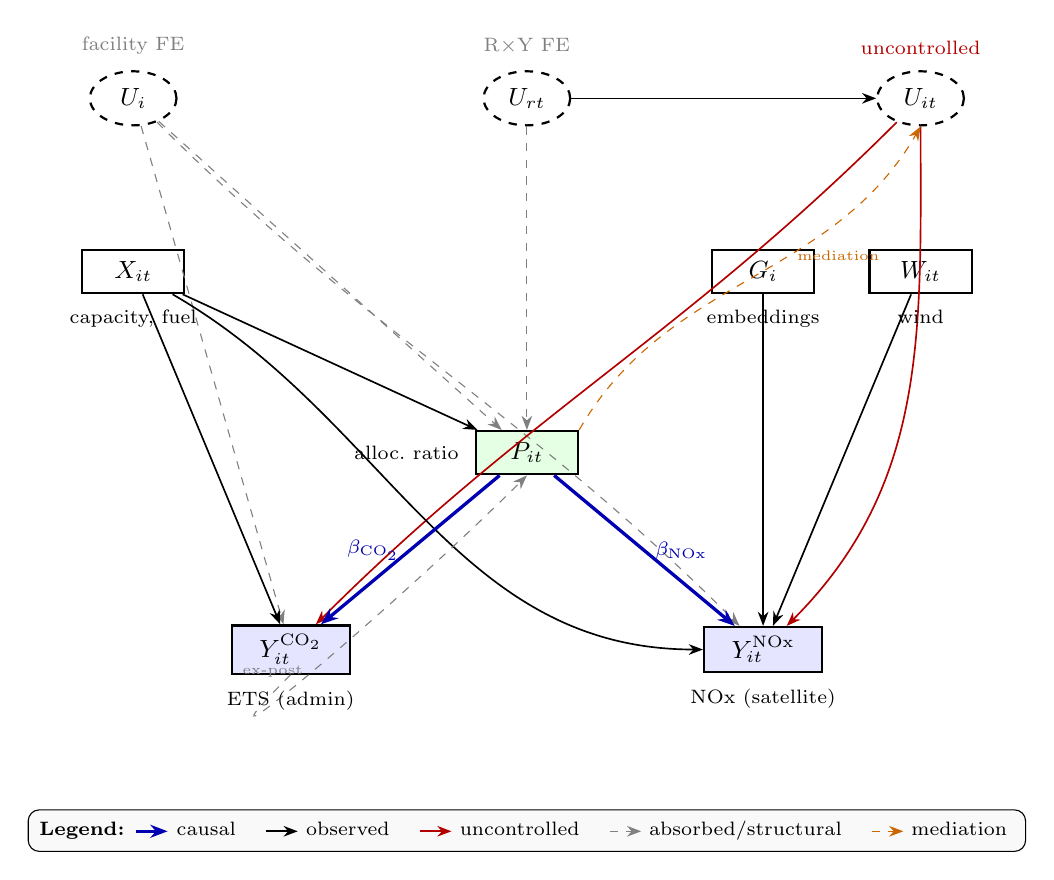
\begin{tikzpicture}[
    observed/.style={rectangle, draw=black, thick, minimum width=1.3cm, minimum height=0.55cm, align=center, font=\small},
    unobserved/.style={ellipse, draw=black, thick, dashed, minimum width=1.1cm, minimum height=0.5cm, align=center, font=\small},
    outcome/.style={rectangle, draw=black, thick, fill=blue!10, minimum width=1.5cm, minimum height=0.55cm, align=center, font=\small},
    treatment/.style={rectangle, draw=black, thick, fill=green!10, minimum width=1.3cm, minimum height=0.55cm, align=center, font=\small},
    arrow/.style={-{Stealth[length=1.8mm]}, semithick},
    dashedarrow/.style={-{Stealth[length=1.8mm]}, thin, dashed, gray},
    redarrow/.style={-{Stealth[length=1.8mm]}, semithick, red!70!black},
    causalarrow/.style={-{Stealth[length=2.2mm]}, very thick, blue!70!black},
    orangearrow/.style={-{Stealth[length=1.8mm]}, thin, dashed, orange!80!black},
]

% === LAYOUT: 3 columns (Left/Center/Right), 4 rows ===
% Coordinates chosen to create clear vertical lanes

% Row 0: Unobserved (y=0)
\node[unobserved] (Ui)  at (-5,   0)   {$U_i$};
\node[unobserved] (Urt) at ( 0,   0)   {$U_{rt}$};
\node[unobserved] (Uit) at ( 5,   0)   {$U_{it}$};

% Row 1: Observed controls (y=-2.2)
\node[observed] (X) at (-5, -2.2) {$X_{it}$};
\node[observed] (G) at ( 3, -2.2) {$G_i$};
\node[observed] (W) at ( 5, -2.2) {$W_{it}$};

% Row 2: Treatment (y=-4.5)
\node[treatment] (P) at (0, -4.5) {$P_{it}$};

% Row 3: Outcomes (y=-7)
\node[outcome] (YCO2) at (-3, -7) {$Y_{it}^{\text{CO}_2}$};
\node[outcome] (YNOx) at ( 3, -7) {$Y_{it}^{\text{NOx}}$};

% =======================================================================
% ARROWS - grouped by type for clarity
% =======================================================================

% --- (A) FACILITY FE: U_i -> P, Y_CO2, Y_NOx (gray dashed, left lane) ---
\draw[dashedarrow] (Ui) -- (P);
\draw[dashedarrow] (Ui) -- (YCO2);
\draw[dashedarrow] (Ui) to[out=-45, in=135] (YNOx);

% --- (B) REGION×YEAR FE: U_rt -> P (gray dashed, center) ---
\draw[dashedarrow] (Urt) -- (P);

% --- (C) UNOBSERVED DYNAMICS: U_rt -> U_it (black, top row) ---
\draw[arrow] (Urt) -- (Uit);

% --- (D) RESIDUAL CONFOUNDING: U_it -> Y_CO2, Y_NOx (red, right lane) ---
\draw[redarrow] (Uit) to[out=-90, in=45] (YNOx);
\draw[redarrow] (Uit) to[out=-135, in=45] (YCO2);

% --- (E) OBSERVED CONTROLS: X -> P, Y_CO2, Y_NOx (black) ---
\draw[arrow] (X) -- (P);
\draw[arrow] (X) -- (YCO2);
\draw[arrow] (X) to[out=-30, in=180] (YNOx);

% --- (F) SATELLITE-ONLY CONTROLS: G, W -> Y_NOx (black, right side) ---
\draw[arrow] (G) -- (YNOx);
\draw[arrow] (W) -- (YNOx);

% --- (G) CAUSAL EFFECTS: P -> Y_CO2, Y_NOx (blue, thick) ---
\draw[causalarrow] (P) -- node[left, font=\scriptsize, pos=0.5] {$\beta_{\text{CO}_2}$} (YCO2);
\draw[causalarrow] (P) -- node[right, font=\scriptsize, pos=0.5] {$\beta_{\text{NOx}}$} (YNOx);

% --- (H) EX-POST RATIO: Y_CO2 -> P (gray dashed, curves left outside) ---
\draw[dashedarrow] (YCO2.south) to[out=-135, in=-135, looseness=1.5] 
    node[left, font=\tiny, pos=0.5] {ex-post} (P.south);

% --- (I) MEDIATION: P -> U_it (orange dashed, curves right outside) ---
\draw[orangearrow] (P.north east) to[out=60, in=-120] 
    node[right, font=\tiny, text=orange!80!black, pos=0.6] {mediation} (Uit.south);

% =======================================================================
% LABELS
% =======================================================================
\node[above=0.08cm of Ui,  font=\scriptsize, gray] {facility FE};
\node[above=0.08cm of Urt, font=\scriptsize, gray] {R$\times$Y FE};
\node[above=0.08cm of Uit, font=\scriptsize, red!70!black] {uncontrolled};

\node[below=0.08cm of X, font=\scriptsize] {capacity, fuel};
\node[below=0.08cm of G, font=\scriptsize] {embeddings};
\node[below=0.08cm of W, font=\scriptsize] {wind};

\node[left=0.08cm of P, font=\scriptsize] {alloc.\ ratio};

\node[below=0.08cm of YCO2, font=\scriptsize] {ETS (admin)};
\node[below=0.08cm of YNOx, font=\scriptsize] {NOx (satellite)};

% =======================================================================
% LEGEND (compact, two rows)
% =======================================================================
\node[draw, rounded corners, fill=gray!5, inner sep=4pt, font=\scriptsize, align=left] at (0, -9.3) {
\textbf{Legend:} 
\tikz[baseline=-0.5ex]{\draw[causalarrow] (0,0) -- (0.4,0);} causal \quad
\tikz[baseline=-0.5ex]{\draw[arrow] (0,0) -- (0.4,0);} observed \quad
\tikz[baseline=-0.5ex]{\draw[redarrow] (0,0) -- (0.4,0);} uncontrolled \quad
\tikz[baseline=-0.5ex]{\draw[dashedarrow] (0,0) -- (0.4,0);} absorbed/structural \quad
\tikz[baseline=-0.5ex]{\draw[orangearrow] (0,0) -- (0.4,0);} mediation
};

\end{tikzpicture}
\caption{Directed acyclic graph for dual-outcome causal inference. Treatment $P_{it}$ (allocation ratio) affects both verified CO$_2$ and satellite NOx outcomes. Gray dashed arrows from $U_i$ and $U_{rt}$ are absorbed by facility and region$\times$year fixed effects, respectively. Red arrows from $U_{it}$ indicate residual confounding from time-varying unobservables (dispatch, maintenance) that we intentionally leave uncontrolled to preserve the mediation pathway (orange). The ex-post arrow reflects that allocation ratios are mechanically computed from prior verified emissions. Observed controls $X_{it}$ (capacity, fuel) affect both outcomes; $G_i$ (embeddings) and $W_{it}$ (wind) affect only the satellite outcome.}\label{fig:dag}
\end{figure}

\subsection{Identification Strategy and Variable Selection}\label{sec:methods:identification}

The identification strategy relies on two key choices: (i) what to control for, and (ii) what \textit{not} to control for. Both are essential to avoid bias.

\subsubsection{Why We Control for Region$\times$Year Effects}

Regional electricity demand, fuel prices, and economic conditions create time-varying confounding: demand shocks increase plant utilization, raising both verified emissions (lowering $R_{it}$) and NO$_2$ output. Without adjustment, this creates spurious correlation between policy stringency and pollution.

Region$\times$Year fixed effects absorb these common shocks additively. The identifying variation becomes: \textit{within the same region and year, do facilities with different allocation ratios exhibit different NO$_2$ enhancement?} This comparison holds regional conditions constant while exploiting cross-facility variation in policy exposure.

I use NUTS2 regions (Nomenclature of Territorial Units for Statistics, level 2) from Eurostat for clustering. NUTS2 regions ($\sim$200--300 across the EU) define economically coherent regional units that share common labor markets, policy enforcement mechanisms, and infrastructure characteristics. Unlike PyPSA-Eur power system clusters (which are appropriate for electricity sector heterogeneity analysis), NUTS2 regions apply to all industrial facility types---power plants, refineries, cement plants---and correspond to administrative units where regional policies are implemented and enforced. This makes them appropriate for absorbing regional time-varying confounders that affect facilities regardless of their sectoral activity.

\subsubsection{Why We Do Not Control for $U_{it}$ (Plant-Level Time-Varying Unobservables)}

Plant-level time-varying unobservables ($U_{it}$) include dispatch/utilization, maintenance status, operational efficiency changes, and idiosyncratic output demand. These variables---particularly dispatch---present a ``bad control'' problem because dispatch is simultaneously:
\begin{enumerate}
    \item \textbf{A confounder}: Demand shocks $\to$ higher dispatch $\to$ higher verified emissions $\to$ lower $R_{it}$. The same shocks $\to$ more combustion $\to$ higher NO$_2$.
    \item \textbf{A potential mediator}: If policy affects merit order bidding (facilities with carbon shortfalls bid higher $\to$ get dispatched less), then: $P_{it} \to U_{it} \to Y_{it}$.
\end{enumerate}

Controlling for $U_{it}$ (or proxies such as generation data) would absorb both effects. The confounding component should be removed, but blocking the mediation pathway would attenuate the true policy effect toward zero. Since we cannot empirically separate these components without strong assumptions about the dispatch mechanism, we do not control for $U_{it}$ directly. Instead, Region$\times$Year FE absorbs the common (regional) component of $U_{it}$---since dispatch responds primarily to regional demand and fuel prices---leaving only facility-specific deviations as residual confounding. These facility-specific deviations are plausibly second-order and orthogonal to the allocation ratio conditional on capacity and fuel mix controls.

\subsubsection{Why Not Facility$\times$Year Fixed Effects?}

Facility$\times$year fixed effects ($\alpha_{it}$) would absorb \textit{all} within-facility-year variation. Since treatment varies at the facility-year level, this leaves no variation to identify $\beta$. More subtly, interactive fixed effects models (which estimate facility-specific responses to common time factors) risk similar problems: if the estimated factor loadings correlate with how allocations were assigned, conditioning on them may open backdoor paths through the allocation mechanism or block mediation pathways.

\subsubsection{Addressing Simultaneity in the Allocation Ratio}

The allocation ratio $R_{it} = A_{it} / V_{it}$ involves current-year verified emissions $V_{it}$ in the denominator, creating apparent simultaneity. However, the \textbf{temporal structure of EU ETS compliance} eliminates this concern. The annual compliance cycle proceeds as follows:
\begin{enumerate}
    \item \textbf{Free allocation granted} (28 February of year $t$): Competent authorities issue free allowances $A_{it}$ to each installation based on predetermined benchmarks \cite{ecets2023revision}.
    \item \textbf{Emissions occur} (throughout year $t$): Facilities make operational decisions---dispatch, fuel choice, maintenance---knowing their allocation $A_{it}$.
    \item \textbf{Emissions verified and reported} (31 March of year $t+1$): Accredited verifiers audit emissions $V_{it}$.
    \item \textbf{Allowances surrendered} (30 April of year $t+1$): Facilities surrender allowances equal to verified emissions.
\end{enumerate}

The key insight is that $A_{it}$ is \textbf{known before} emissions decisions are made. Facilities observe their allocation at the start of the year and adjust operations accordingly. The causal direction is unambiguous: $A_{it} \to \text{decisions} \to V_{it}$. The dashed arrow from $Y_{it}^{\text{CO}_2}$ to $P_{it}$ in Figure~\ref{fig:dag} represents the ex-post calculation of the ratio, not reverse causation within the compliance period.

Within the econometric design, Region$\times$Year FE absorbs common drivers of dispatch variation (carbon prices, regional demand, fuel prices). The remaining cross-facility variation in $R_{it}$ within a region-year reflects primarily differences in predetermined allocations $A_{it}$ rather than differences in current dispatch.

To the extent that endogenous dispatch variation contaminates $R_{it}$ through the denominator, the bias is likely \textit{attenuating}: facilities with high dispatch have both lower allocation ratios (higher denominator) and higher emissions, creating positive correlation between $R_{it}$ and $Y_{it}$ that works against finding a negative policy effect. Estimates should therefore be interpreted as conservative.

\subsubsection{Residual Threats and Interpretation}

The primary residual threat is facility-specific time-varying confounding ($U_{it}$)---maintenance outages, unexpected efficiency changes, or idiosyncratic demand for a specific plant's output. These are plausibly second-order and unlikely to systematically correlate with allocation ratios conditional on our controls. Future work incorporating plant-level generation data could address this directly; a discussion of economic dispatch and power system optimization is reserved for subsequent analysis.

\subsubsection{Outcome-Specific Controls}\label{sec:methods:outcome-specific}

Two variables affect only the satellite NOx outcome, not verified ETS CO$_2$:

\begin{itemize}
    \item \textbf{Wind ($W_{it}$)}: The Beirle flux-divergence method uses wind speed and direction to compute advected NO$_2$ mass flux. Wind enters the satellite \textit{measurement process}---it does not affect actual emissions or administrative reporting.
    \item \textbf{AlphaEarth embeddings ($G_i$)}: Geographic context (terrain, land use, climate) affects satellite retrieval quality---terrain influences air mass factor corrections; urban land use creates background NO$_2$ that adds noise to point-source signals; climate affects atmospheric dispersion and NOx lifetime. None of these affect the administrative mass-balance calculation underlying ETS CO$_2$.
\end{itemize}

For ETS CO$_2$, geographic confounders are absorbed by facility fixed effects (time-invariant factors like location, baseline technology) and region$\times$year fixed effects (time-varying regional factors). Including embeddings for the ETS outcome would control for variation irrelevant to that measurement process.

\subsubsection{Embedding Dimensionality Reduction}\label{sec:methods:embedding-reduction}

The raw AlphaEarth embeddings (64 dimensions) may introduce overfitting concerns in the TWFE specification, particularly when the panel contains limited within-facility variation. Two dimensionality reduction strategies are considered:

\textbf{PCA (unsupervised)}: Standard principal component analysis projects embeddings onto directions that maximize variance in the embedding space. This is causally safe because it does not use outcome information---the projection is determined entirely by the covariate distribution.

\textbf{Facility-level PLS (supervised)}: Partial least squares regression projects embeddings onto directions that predict the outcome. However, naive application of PLS to panel data creates \textit{regularization bias}: the learned projection incorporates information from year-specific outcome shocks, violating the requirement that controls be pre-determined \cite{chernozhukov2018}. This is analogous to the ``bad controls'' problem identified by \cite{cinelli2022}: if the projection learns to predict treatment-affected variation in the outcome, controlling for the reduced embeddings biases the treatment effect estimate.

I address this by training PLS on \textbf{facility-level means} (one observation per facility) rather than panel observations. Let $\bar{Y}_i^{\text{NOx}} = T^{-1} \sum_t Y_{it}^{\text{NOx}}$ denote the time-averaged NOx emission rate for facility $i$. The PLS projection is learned from the cross-sectional regression:
\begin{equation}
\bar{Y}_i^{\text{NOx}} = \mathbf{e}_i' \boldsymbol{\gamma} + \eta_i
\label{eq:pls_training}
\end{equation}
where $\mathbf{e}_i \in \mathbb{R}^{64}$ is the embedding vector and $\boldsymbol{\gamma}$ are PLS loadings. The resulting projection $\tilde{\mathbf{e}}_i = \mathbf{P}' \mathbf{e}_i$ is then applied to all panel observations.

This design ensures the reduced embeddings are \textit{time-invariant} within each facility, making them equivalent to pre-treatment covariates. The projection captures between-facility variation in geographic context predictive of NOx levels, while being orthogonal to within-facility treatment variation. This is analogous to the sample-splitting approach in double/debiased machine learning \cite{chernozhukov2018}, where nuisance parameters are estimated on auxiliary data to prevent overfitting bias.

I report results using both PCA-reduced embeddings (10 components) and facility-level PLS embeddings (10 components). Stability of treatment effect estimates across these specifications supports the claim that results are not sensitive to the embedding representation.

\subsection{Treatment Definitions}\label{sec:methods:treatment}

\subsubsection{Continuous Treatment}

The primary treatment variable is the allocation ratio $R_{it}$ (Equation~\ref{eq:allocratio}). Lower values indicate greater policy stringency---facilities must purchase more allowances on the carbon market when $R_{it} < 1$. The expected effect is that lower allocation ratios induce emissions reductions, leading to lower verified CO$_2$ and correspondingly lower satellite-derived NOx (as NOx is a combustion co-pollutant).

\subsubsection{Discrete Treatment for Staggered DiD}

For the Callaway-Sant'Anna estimator, I define a binary treatment indicator:
\begin{equation}
D_{it} = \mathbf{1}\{R_{it} < 1\}
\label{eq:treated}
\end{equation}
where $\mathbf{1}\{\cdot\}$ is the indicator function. Treatment onset (cohort assignment) is defined as the first year a facility becomes treated:
\begin{equation}
G_i = \min\{t : D_{it} = 1\}
\label{eq:cohort}
\end{equation}
Facilities never treated are assigned $G_i = 0$ (the never-treated control group).

\subsection{TWFE with Continuous Treatment}\label{sec:methods:twfe}

The main two-way fixed effects specification uses facility and region$\times$year fixed effects:
\begin{equation}
Y_{it} = \alpha_i + \gamma_{r(i),t} + \beta R_{it} + \mathbf{X}_{it}'\boldsymbol{\delta} + \varepsilon_{it}
\label{eq:twfe}
\end{equation}
where:
\begin{itemize}
    \item $\alpha_i$: Facility fixed effects (absorb time-invariant unobservables)
    \item $\gamma_{r(i),t}$: Region$\times$Year fixed effects, where $r(i)$ denotes the NUTS2 region containing facility $i$ (absorb regional time-varying confounders)
    \item $\beta$: Treatment effect of interest (effect of unit increase in allocation ratio)
    \item $\mathbf{X}_{it}$: Time-varying controls (capacity, fuel shares) and static AlphaEarth embedding controls ($\mathbf{e}_i \in \mathbb{R}^{64}$)
    \item $\varepsilon_{it}$: Idiosyncratic error
\end{itemize}

This specification absorbs all region-specific time-varying confounders, including regional electricity prices, demand conditions, fuel prices, and policy enforcement intensity. Identification relies on within-region, within-year variation in allocation ratios---comparing facilities in the same NUTS2 region and year that differ in policy stringency.

The coefficient $\beta$ is identified from within-facility variation in allocation ratios over time, after controlling for region-year effects. For the CO$_2$ outcome, a positive $\beta$ would indicate that higher allocation ratios (less policy stringency) are associated with higher verified emissions---equivalently, that policy stringency reduces CO$_2$. For the NOx outcome, a positive $\beta$ would indicate corresponding reductions in satellite-derived NOx, consistent with co-pollutant dynamics.

Standard errors are clustered at the NUTS2 region level. NUTS2 regions ($\sim$200--300 across the EU) define economically coherent regional units that share common labor markets, policy enforcement mechanisms, and infrastructure characteristics.

\subsection{Callaway-Sant'Anna Difference-in-Differences}\label{sec:methods:csdid}

The Callaway and Sant'Anna \cite{callaway2021} estimator addresses potential bias in standard TWFE when treatment timing varies across units and treatment effects are heterogeneous. The method estimates group-time average treatment effects:
\begin{equation}
ATT(g,t) = \mathbb{E}[Y_{it}(1) - Y_{it}(0) \mid G_i = g]
\label{eq:attgt}
\end{equation}
for each cohort $g$ (first treatment year) and calendar time $t$.

Key features of the implementation:
\begin{itemize}
    \item \textbf{Control group}: Never-treated units (facilities with $R_{it} \geq 1$ in all years)
    \item \textbf{Estimation method}: Doubly robust (combining outcome regression and propensity score weighting)
    \item \textbf{Anticipation}: Zero (no anticipation effects assumed)
\end{itemize}

The group-time ATTs are aggregated to produce:
\begin{enumerate}
    \item \textbf{Simple aggregate ATT}: Overall average treatment effect across all treated observations:
    \begin{equation}
    ATT^{\text{simple}} = \sum_{g} \sum_{t \geq g} w_{g,t} \cdot ATT(g,t)
    \label{eq:attsimple}
    \end{equation}
    \item \textbf{Dynamic/event-study ATT}: Effects by time relative to treatment:
    \begin{equation}
    ATT(e) = \sum_{g} w_g \cdot ATT(g, g+e)
    \label{eq:attevent}
    \end{equation}
    where $e$ is event time (years since treatment onset)
\end{enumerate}

The event-study specification enables pre-trend testing: under parallel trends, $ATT(e) = 0$ for $e < 0$. A Wald test of joint nullity for pre-treatment periods provides formal evidence on the parallel trends assumption.

\subsection{NUTS2-Based Clustering for Inference}\label{sec:methods:clustering}

Standard errors are clustered at the NUTS2 region level throughout. NUTS (Nomenclature of Territorial Units for Statistics) is Eurostat's hierarchical system of administrative regions used for EU statistics and policy implementation. NUTS2 regions ($\sim$200--300 across the EU) correspond to basic regions for the application of regional policies, typically containing 800,000 to 3 million inhabitants.

NUTS2 regions are appropriate clustering units because they define economically coherent areas where:
\begin{itemize}
    \item \textbf{Common policy enforcement}: EU and national environmental regulations are implemented and enforced at regional administrative levels
    \item \textbf{Shared labor markets}: Facilities in the same NUTS2 region draw from similar labor pools and face similar wage pressures
    \item \textbf{Correlated economic conditions}: Regional GDP, industrial activity, and energy demand co-move within administrative regions
\end{itemize}

Unlike sector-specific clustering (e.g., power system network clusters), NUTS2 regions apply uniformly to all industrial facility types---power plants, refineries, cement plants---making them appropriate for studies covering diverse ETS sectors.

\subsubsection{PyPSA-Eur Clusters for Electricity Sector Heterogeneity}

For electricity sector heterogeneity analysis, I additionally implement PyPSA-Eur power system clusters \cite{horsch2018}, which are \textit{not} geographic or administrative regions but rather k-means clusters computed directly on power system features extracted from the European high-voltage transmission network (ENTSO-E data), solved using the Gurobi optimizer \cite{gurobi}. The clustering algorithm groups electrical buses (substations) based on network connectivity, line impedances, and transmission capacity. The objective function minimizes within-cluster electrical distance, producing clusters where facilities face similar grid constraints, transmission losses, and wholesale price dynamics.

This clustering approach has a theoretical justification grounded in recent work on network cluster-robust inference. \cite{kojevnikov2023} establish that valid cluster-robust standard errors require clusters with low ``conductance''---formally, the ratio of edges crossing cluster boundaries to total within-cluster edges. The k-means clustering on transmission network features directly minimizes this quantity: by grouping buses to minimize within-cluster electrical distance (impedance), the algorithm produces clusters with few high-capacity transmission lines crossing boundaries. Facilities within the same cluster are therefore more strongly connected to each other (through the grid) than to facilities in other clusters, satisfying the theoretical requirements for cluster-robust inference.

This represents a novel application of model-derived clustering for econometric inference. Rather than using geographic proximity (which ignores network topology), administrative boundaries (which may cut across electrically-connected regions), or data-driven clustering on outcome variables (which risks overfitting), I use clusters computed from features of an external domain-specific model---the power system transmission network---that captures the economically-relevant correlation structure a priori. For this analysis, the 128-region resolution is used, providing sufficient granularity to capture sub-national variation while maintaining adequate within-region sample sizes for clustered inference. Each facility is assigned to the PyPSA-Eur cluster containing the nearest network bus.

Let $r \in \{1, \ldots, R\}$ index NUTS2 regions. The cluster-robust variance estimator for the TWFE coefficient is:
\begin{equation}
\widehat{\text{Var}}(\hat{\beta}) = \left(\mathbf{X}'\mathbf{M}\mathbf{X}\right)^{-1} \left(\sum_{r=1}^{R} \mathbf{X}_r'\hat{\mathbf{u}}_r\hat{\mathbf{u}}_r'\mathbf{X}_r\right) \left(\mathbf{X}'\mathbf{M}\mathbf{X}\right)^{-1}
\label{eq:clustervar}
\end{equation}
where $\mathbf{M}$ is the residual maker for fixed effects and $\hat{\mathbf{u}}_r$ are residuals for observations in NUTS2 region $r$.

\subsection{Summary of Specifications}\label{sec:methods:summary}

Table~\ref{tab:specs} summarizes the six core specifications estimated in this study. The dual-outcome design combined with two estimators and two embedding strategies for the satellite outcome yields six specifications.

\begin{table}[h]
\caption{Summary of Econometric Specifications}\label{tab:specs}%
\begin{tabular*}{\textwidth}{@{\extracolsep\fill}clll}
\toprule
Spec & Outcome & Embedding Strategy & Estimator \\
\midrule
1 & ETS CO$_2$ & None & TWFE \\
2 & ETS CO$_2$ & None & Callaway-Sant'Anna \\
3 & Satellite NOx & PCA (10 dims) & TWFE \\
4 & Satellite NOx & PCA (10 dims) & Callaway-Sant'Anna \\
5 & Satellite NOx & PLS (10 dims) & TWFE \\
6 & Satellite NOx & PLS (10 dims) & Callaway-Sant'Anna \\
\botrule
\end{tabular*}
\footnotetext{Note: ETS CO$_2$ uses no embeddings because geographic context does not affect administrative data measurement. For satellite NOx, PCA provides an unsupervised (outcome-agnostic) projection while PLS provides a supervised projection trained on facility-level mean NOx to ensure causal validity. All specifications use Facility + Region$\times$Year fixed effects and cluster standard errors by NUTS2 region.}
\end{table}

%% ========================================================================
%% RESULTS
%% ========================================================================
\section{Results}\label{sec:results}

\textit{[Results to be added upon completion of empirical analysis.]}

This section will present:
\begin{enumerate}
    \item Descriptive statistics on treatment and outcome distributions
    \item Estimates for all six specifications (Table~\ref{tab:specs})
    \item Callaway-Sant'Anna event study results with pre-trend tests
    \item Comparison of CO$_2$ and NOx responses: agreement in sign and magnitude
    \item Stability of results across embedding strategies (PCA vs PLS)
\end{enumerate}

\subsection{Treatment Distribution}

The allocation ratio exhibits substantial within-facility variation over the sample period. [Distribution statistics and figures to be added.]

\subsection{Main Estimates}

Table~\ref{tab:main} reports the main estimation results.

\begin{table}[h]
\caption{Main Estimation Results: Effect of Allocation Ratio on Dual Outcomes}\label{tab:main}%
\begin{tabular*}{\textwidth}{@{\extracolsep\fill}lcc}
\toprule
& Verified CO$_2$ (ktCO$_2$/yr) & Satellite NOx (kg/s) \\
\midrule
Allocation Ratio ($R_{it}$) & [--] & [--] \\
& ([--]) & ([--]) \\
\midrule
Facility FE & Yes & Yes \\
Region$\times$Year FE & Yes & Yes \\
Controls & Yes & Yes \\
\midrule
Observations & [--] & [--] \\
Facilities & [--] & [--] \\
$R^2$ (within) & [--] & [--] \\
\botrule
\end{tabular*}
\footnotetext{Note: Standard errors clustered by NUTS2 region in parentheses. Controls include capacity (MW), fuel shares (coal, gas), and AlphaEarth embeddings (64 dimensions). * $p<0.10$, ** $p<0.05$, *** $p<0.01$.}
\end{table}

\subsection{Event Study}

Figure~\ref{fig:eventstudy} presents the Callaway-Sant'Anna event study results for both outcomes, plotting dynamic treatment effects by years relative to treatment onset. Comparison of CO$_2$ and NOx event-study patterns provides a cross-validation of policy effects: if carbon pricing reduces combustion, both outcomes should show similar post-treatment declines.

[Event study figure to be added.]

Pre-trend tests: [Wald test results to be added.]

\subsection{Robustness}

[Robustness analysis to be added, including:]
\begin{itemize}
    \item Alternative emissions thresholds (250 kt, 500 kt)
    \item Alternative treatment definitions (shortfall instead of ratio)
    \item Heterogeneity by fuel type and country
    \item Sensitivity to NOx detection limit (excluding facilities below 0.11 kg/s)
    \item Comparison of CO$_2$ vs NOx elasticities (percentage changes)
\end{itemize}

%% ========================================================================
%% DISCUSSION
%% ========================================================================
\section{Discussion}\label{sec:discussion}

\textit{[Discussion to be completed with empirical results.]}

This study develops a methodological framework for evaluating climate policy impacts using dual outcomes: verified EU ETS CO$_2$ emissions and satellite-derived NOx emission proxies. This approach enables comprehensive assessment of both greenhouse gas reductions and air quality co-benefits. Several aspects merit discussion.

\subsection{Interpretation of Estimates}

The allocation ratio treatment variable has a natural interpretation in terms of policy stringency. A coefficient estimate of $\beta$ on $R_{it}$ implies that a 0.1 unit decrease in the allocation ratio (from 1.0 to 0.9, representing a shift from full free allocation to 10\% shortfall) is associated with a $-0.1\beta$ change in the outcome variable.

\textbf{For verified CO$_2$}: The outcome is directly measured and reported under EU ETS compliance, providing high-quality estimates of policy effects on greenhouse gas emissions.

\textbf{For satellite-derived NOx}: The Beirle-style flux-divergence approach provides a metric that is physically grounded in the continuity equation, with advection proportional to local emissions minus chemical sinks. Unlike simple column density comparisons, this method isolates facility-attributable emissions from regional background. However, interpretation requires caution due to the substantial uncertainty components discussed in Section~\ref{sec:data:beirle}.

\textbf{Cross-validation}: Agreement in sign and broad magnitude between CO$_2$ and NOx responses provides confidence that both outcomes are capturing genuine policy effects. Perfect correspondence is not expected---NOx and CO$_2$ have different emission factors by fuel type and combustion conditions---but directional agreement supports the validity of both measures.

\subsection{Identification Concerns}

Several potential threats to identification remain. First, \textbf{operational confounding}: facilities may respond to high carbon prices by adjusting operations (reducing output, switching fuels) in ways that are not fully captured by the control variables. To the extent that these operational responses are the mechanism through which carbon pricing affects air quality, this is not problematic---it is the causal effect of interest. However, if operational changes are driven by other factors correlated with allocation ratios (e.g., electricity prices), bias may result.

Second, \textbf{measurement error in satellite NOx}: The Beirle-style flux-divergence approach is subject to multiple uncertainty sources (Section~\ref{sec:data:beirle}): lifetime parameterization (50\% relative uncertainty), product differences between OFFL and PAL ($\pm$25\%), NOx/NO$_2$ scaling ($\sim$7\%), and spatial integration noise. These compound to total uncertainties of 20--40\% per facility-year, with potential systematic low bias of $\sim$20\% relative to reported emissions. This measurement error attenuates treatment effect estimates toward zero, making the satellite-based findings conservative.

Third, \textbf{spillovers}: if carbon pricing induces substitution across facilities (e.g., shifting generation from high-cost to low-cost plants), the stable unit treatment value assumption (SUTVA) may be violated. The region$\times$year fixed effects specification partially addresses this by absorbing regional substitution patterns.

\subsection{Limitations of the Satellite NOx Proxy}

The satellite-derived NOx estimates should be interpreted with several limitations in mind:
\begin{itemize}
    \item \textbf{Use of OFFL L3 instead of PAL}: Beirle et al. (2023) use the PAL NO$_2$ product, which provides 10--40\% higher TVCDs. The OFFL L3 product available via Google Earth Engine introduces additional uncertainty.
    \item \textbf{Simplified NOx/NO$_2$ scaling}: The photostationary-state approximation may not hold near stack plumes; I apply a fixed ratio of 1.38 $\pm$ 0.10 following Beirle et al. (approximately 7\% uncertainty).
    \item \textbf{Integration radius trade-off}: The 15 km radius balances capturing the full point source signal against spatial interference from neighboring sources. For facilities in dense industrial areas, some signal contamination is likely.
    \item \textbf{Spatial interference}: For facilities with another ETS facility within 20~km (flagged via \texttt{interfered\_20km}), the satellite outcome reflects emissions of the \textit{local cluster} rather than an isolated point source. Treatment effect estimates for these facilities should be interpreted as cluster-level responses. Sensitivity analyses excluding interfered facilities test whether results are robust to this contamination.
    \item \textbf{Detection limit}: Beirle et al. Sect. 3.11.1 report detection limits of 0.11 kg/s (standard conditions) down to 0.03 kg/s (ideal high-albedo conditions). Since we do not implement a surface reflectivity mask, we flag observations against both thresholds and present sensitivity analysis using the conservative 0.11 kg/s threshold for Europe.
    \item \textbf{Skipping automatic identification}: We skip Beirle's automatic point-source identification algorithm because we have known ETS/LCP source locations. This design choice is explicitly endorsed by the authors and is conceptually appropriate for our use case, but it means we do not benefit from their classification step that filters artifacts and non-point sources. To compensate, we apply simplified significance filters (detection limit, statistical integration error, interference flag).
    \item \textbf{Unmodeled corrections}: AMF correction and plume height effects following Beirle et al. (2023) are not fully implemented, contributing to structural uncertainty. Topographic correction is implemented using SRTM elevation data.
    \item \textbf{Temporal averaging approach}: Beirle et al. compute temporal means of A* at orbit resolution before applying a single lifetime correction using mean wind speed. I instead aggregate to daily resolution and apply the lifetime correction per-day before temporal averaging, i.e., $E = \text{mean}[c_\tau(w_d) \times A^*_d]$ rather than $c_\tau(\bar{w}) \times \text{mean}(A^*)$. Since $c_\tau$ is nonlinear in wind speed, these are not mathematically identical; however, the difference is small for typical wind speed variance and the per-day approach is more appropriate for constructing annual panel estimates rather than a single multi-year catalog value.
\end{itemize}

These design choices---using OFFL instead of PAL, simplified significance flags, skipping the automatic identification algorithm---primarily increase noise and potential attenuation bias, not spurious detection. The satellite outcome remains a \textit{physically grounded but noisy proxy}; ETS verified CO$_2$ remains the primary outcome for causal inference.

\subsection{Methodological Contributions: ML-Derived Features in Causal Inference}

This study contributes to a growing literature on incorporating machine learning-derived features into causal inference frameworks \cite{chernozhukov2018,veitch2019,zimmert2018}. Two aspects merit particular discussion.

\textbf{Geospatial foundation model embeddings as controls.} The use of AlphaEarth embeddings \cite{alphaearth2025} demonstrates that pre-trained geospatial representations can serve as effective high-dimensional controls in panel settings. Unlike manually-specified geographic controls (distance to coast, elevation, population density), foundation model embeddings capture complex, nonlinear combinations of features that the model learned to be predictive across diverse tasks. The key assumption---that these embeddings capture confounders affecting both policy exposure and air quality outcomes---is plausible given that the embeddings encode land use, infrastructure, and climate patterns that likely correlate with both industrial activity and pollution dispersion. Future work should investigate the sensitivity of causal estimates to different embedding specifications and the conditions under which learned representations provide valid confounding adjustment.

\textbf{Network-based clustering from external models.} The use of PyPSA-Eur power system clusters for both fixed effects and inference represents a novel application of model-derived features for econometric analysis. Traditional approaches to clustered standard errors use geographic proximity or administrative boundaries that may not reflect the economically-relevant correlation structure. By using clusters derived from transmission network topology \cite{horsch2018}, which minimize within-cluster electrical distance, I define regions where facilities face correlated prices, dispatch patterns, and demand shocks---precisely the correlations that motivate cluster-robust inference \cite{kojevnikov2023}. This approach could be extended to other networked industries where external models of the network structure are available.

\subsection{Limitations and Future Work}

\textbf{Sample attrition.}
The requirement for valid linkage across three independent data sources (LCP registry, EU Registry crosswalk, EUTL compliance data) reduces the initial universe of 3,405 LCP plants to 521 facilities (15.3\% retention). The satellite NOx outcome will have additional attrition from detection limits and observation coverage requirements. This attrition reduces statistical power and may introduce selection bias if the matched sample differs systematically from the broader LCP population. The 500m spatial clustering threshold, while appropriate for grouping co-located emission sources into coherent facilities, may occasionally merge distinct plants or fail to group plants that share a common plume.

\textbf{Size threshold and generalizability.}
The sample is restricted to large facilities with sufficient emissions for satellite detection (0.11 kg/s NOx conservative threshold), limiting generalizability to smaller sources. The annual temporal resolution may miss short-run dynamics such as seasonal fuel switching or within-year operational adjustments.

\textbf{Satellite measurement uncertainty.}
The satellite NOx proxy is subject to the multiple uncertainty components detailed in Section~\ref{sec:data:beirle}, though these primarily introduce classical measurement error that attenuates rather than biases estimates.

\textbf{Heterogeneous satellite observation coverage.}
Different facilities have different numbers of valid observation days per year (typically 60--80 out of $\sim$180 days with TROPOMI coverage) due to cloud cover, wind speed filtering ($\geq$2 m/s requirement), and satellite orbit patterns. This heterogeneity raises a potential methodological concern: if the subset of observable days differs systematically across facilities---e.g., coastal plants observed more frequently in winter, inland plants more in summer---then annual mean emission rates may not be directly comparable across locations. For panel regressions, this concern is mitigated if: (i) observation selection is driven by weather, which is exogenous to treatment; (ii) the selection mechanism is stable within-facility over time, so facility fixed effects absorb level differences; and (iii) year fixed effects absorb common temporal patterns. As a robustness check, I include the number of valid observation days (\texttt{n\_days\_satellite}) as a control variable; stability of treatment effect estimates with and without this control supports the assumption that observation heterogeneity does not induce substantial bias.

\textbf{UK exclusion.}
The EU ETS registry data used in this study does not include installations in the United Kingdom following Brexit. The UK withdrew from the EU ETS on January 1, 2021, and established its own UK Emissions Trading Scheme \cite{ukgov2024ukets}. Consequently, UK large combustion plants---which represented a significant share of EU ETS-regulated capacity prior to 2021---are excluded from the analysis panel. Future work extending this framework to include UK facilities would require obtaining compliance data from the UK ETS registry and harmonizing it with the EU data sources used here. This may be facilitated in the near future by the linking of the UK and EU's ETS systems.

%% ========================================================================
%% CONCLUSION
%% ========================================================================
\section{Conclusion}\label{sec:conclusion}

This study develops and demonstrates a novel framework for comprehensively evaluating climate policy impacts using dual emission outcomes. By linking administrative EU ETS compliance data with satellite-derived NOx emission proxies constructed via the Beirle-style flux-divergence method, I construct a facility-level panel that enables causal inference on how carbon market stringency affects both verified CO$_2$ emissions and satellite-observable combustion co-pollutants.

The study makes three methodological contributions, two of which follow a recent trend in causal inference toward incorporating machine learning-derived features to address high-dimensional confounding \cite{chernozhukov2018,veitch2019,zimmert2018}.

\textbf{First}, I demonstrate the integration of geospatial foundation model embeddings as high-dimensional controls in panel-based climate monitoring studies. Using Google AlphaEarth \cite{alphaearth2025}---64-dimensional representations learned from multi-source satellite imagery, climate reanalysis, and geotagged text---I capture between-unit heterogeneity arising from local geographic, infrastructural, and climate context in a data-efficient manner. This extends prior work on learned embeddings for causal inference \cite{veitch2019} from text to the geospatial domain, and is particularly relevant for difference-in-differences settings where high-dimensional spatial confounders may violate parallel trends if left uncontrolled \cite{zimmert2018}.

\textbf{Second}, I introduce network-based clustering derived from an external power system model for econometric inference. Standard errors are clustered using PyPSA-Eur power system clusters \cite{horsch2018}---k-means clusters computed on transmission network topology features---that group facilities facing correlated wholesale prices, dispatch patterns, and grid constraints. This approach is grounded in recent theoretical foundations showing that valid cluster-robust inference requires low-conductance clusters \cite{kojevnikov2023}, which network-derived clusters satisfy by construction. To my knowledge, this represents the first application of model-derived clustering---where clusters are computed on features from an external domain-specific model rather than on the outcome data itself---for econometric inference in policy evaluation.

\textbf{Third}, for the satellite outcome, I implement a simplified Beirle-style flux-divergence method that provides physically grounded NOx emission estimates at the facility level. By computing the advection---the wind-aligned spatial derivative of NO$_2$ column density---and integrating over a 15 km disc with lifetime correction, this approach provides facility-specific NOx estimates suitable for panel econometric analysis. This methodology is grounded in the continuity equation and follows the approach of Beirle et al. (2019, 2021, 2023) \cite{beirle2019,beirle2021,beirle2023}, which has been validated against reported emissions from regulatory agencies.

[Substantive empirical conclusions to be added with results.]

The broader contribution of this work is demonstrating that combining administrative emissions records with satellite-derived proxies, along with ML-derived controls and network-informed inference, can provide comprehensive evaluation of climate policy impacts at the individual emitter level. The dual-outcome approach offers several advantages: (i) verified CO$_2$ provides the gold standard for measuring policy effects on greenhouse gas output; (ii) satellite-derived NOx provides an independent check on combustion activity and enables testing co-benefit hypotheses; and (iii) agreement between outcomes provides cross-validation that both measures are capturing genuine policy effects.

As satellite instruments improve in resolution and retrieval accuracy, and as methods like the Beirle flux-divergence approach become more refined, this framework could enable near-real-time monitoring of both carbon and co-pollutant emissions from regulated facilities. Future work could extend this framework to methane point sources (using TROPOMI CH$_4$), investigate heterogeneity across plant types and regulatory contexts, and further develop the theoretical foundations for using learned representations and model-derived clusters in causal inference.

\backmatter

\bmhead{Acknowledgements}

\section*{Declarations}

\begin{itemize}
\item \textbf{Data availability}: EEA Large Combustion Plant data available from the European Environment Agency Industrial Emissions Portal. EU ETS data available from the European Union Transaction Log. TROPOMI data available via Google Earth Engine. ERA5-Land data available from the Copernicus Climate Data Store.
\item \textbf{Code availability}: Full data processing and analysis code available at https://github.com/arnava13/Masters-Thesis
\item \textbf{Use of Generative AI}: Generative AI was used for programming, researching and writing
this paper. Project direction was driven by me, and I manually audited \& corrected all code, sources, citations, equations and theoretical assertions.
\end{itemize}

\begin{appendices}

\section{Data Pipeline Details}\label{app:pipeline}

\subsection{ID Normalization for ETS Linking}

Linking LCP plants to ETS installations requires normalizing identifiers from different sources. EU Registry identifiers follow patterns such as \texttt{FR000000000210535} (padded numeric) or \texttt{FR-new-07101261} (new format). Pyeutl installation IDs follow the format \texttt{AT\_200165} (country code underscore numeric).

The normalization procedure:
\begin{enumerate}
    \item Extract country code (first 2 characters)
    \item Extract all numeric substrings
    \item Select longest numeric substring, strip leading zeros
    \item Combine as \texttt{CC\_NNN} format
\end{enumerate}

This procedure successfully matches 799 of 932 facilities (85.7\%) to ETS installations.

\subsection{Electricity Sector Classification}

Electricity-sector facilities are identified using EU ETS activity codes from the EUTL database, as defined in Directive 2003/87/EC Annex I \cite{euets2003directive,eea2021etsbackground}. Activity codes changed between EU ETS phases:
\begin{itemize}
    \item \textbf{Phases 1--2 (2005--2012)}: Activity Code 1 = ``Combustion installations with a rated thermal input exceeding 20 MW''
    \item \textbf{Phase 3+ (2013--present)}: Activity Code 20 = ``Combustion of fuels''
\end{itemize}

Strictly speaking, these activity codes identify \textit{combustion installations} broadly---including power plants, combined heat and power (CHP), industrial boilers, and district heating---rather than electricity generators specifically. However, for the Large Combustion Plant (LCP) registry used in this study, the sample predominantly comprises electricity-generating facilities. A facility is classified as electricity-sector if it has \textit{any} installation linked to activity codes 1 or 20. This classification is used for electricity-sector heterogeneity analysis employing PyPSA-Eur power system clusters.

\subsection{Fuel Type Classification}

Raw LCP fuel types are mapped to standardized categories:
\begin{itemize}
    \item \textbf{Gas}: NaturalGas, NG, Gas
    \item \textbf{Coal}: Coal, Lignite, PC, BIT, SUB, ANT
    \item \textbf{Oil}: LiquidFuels, DFO, RFO, KER
    \item \textbf{Biomass}: Biomass, WDL, WDS, AB
    \item \textbf{Other Gas}: OtherGases, OBG
\end{itemize}

Fuel types used by fewer than 10\% of facility-years (Other Solid, Peat) are dropped, shares renormalized, and facilities with no remaining fuel coverage are excluded from the sample.

\section{Sample Attrition}\label{app:attrition}

Table~\ref{tab:attrition} summarizes the sample attrition through each processing step. The most significant losses occur at the ETS linkage stage (44\% of plants lack matched ETS identifiers in the EU Registry crosswalk) and the requirement for matched ETS compliance data with valid allocation ratios.

\begin{table}[h]
\caption{Sample Attrition Through Data Processing Pipeline}\label{tab:attrition}%
\begin{tabular*}{\textwidth}{@{\extracolsep\fill}lrrr}
\toprule
Processing Step & Plants/Facilities & Lost & Retained \% \\
\midrule
\multicolumn{4}{l}{\textit{Plant-Level Processing}} \\
\quad Initial LCP registry ($\geq$50 MW thermal) & 3,405 plants & --- & 100\% \\
\quad With complete capacity + fuel data (2018--2023) & 2,821 & 584 & 82.8\% \\
\quad With ETS linkage (via EU Registry crosswalk) & 1,580 & 1,241 & 46.4\% \\
\midrule
\multicolumn{4}{l}{\textit{Facility-Level Processing (after 500m spatial clustering)}} \\
\quad After spatial clustering & 932 facilities & --- & --- \\
\quad With matched ETS compliance data & 608 & 324 & 65.2\% \\
\quad With $\geq$3 years complete data & 521 & 87 & 55.9\% \\
\midrule
\textbf{Base analysis panel (ETS CO$_2$ outcome)} & \textbf{521 facilities} & & \textbf{15.3\%} \\
 & \textbf{2,819 fac-years} & & \textbf{of initial plants} \\
\midrule
\multicolumn{4}{l}{\textit{Additional NOx Outcome Filters}} \\
\quad With satellite data ($\geq$20 valid days/year) & 291 & 230 & 55.9\% \\
\quad With $\leq$50\% total uncertainty & 291 & 0 & 55.9\% \\
\midrule
\textbf{Satellite NOx panel} & \textbf{291 facilities} & & \textbf{8.5\%} \\
 & \textbf{1,213 fac-years} & & \textbf{of initial plants} \\
\botrule
\end{tabular*}
\footnotetext{Note: LCP registry includes only plants with rated thermal input $\geq$50 MW. ETS linkage uses normalized identifier matching between EU Registry and EUTL compliance data. The satellite NOx panel filters on observation coverage ($\geq$20 valid days/year) and total uncertainty ($\leq$50\%). Detection limit (0.11 kg/s) is not used as a sample filter but is reported as a quality indicator.}
\end{table}

\end{appendices}

%%===========================================================================================%%
%% If you are submitting to one of the Nature Portfolio journals, using the eJP submission   %%
%% system, please include the references within the manuscript file itself. You may do this  %%
%% by copying the reference list from your .bbl file, paste it into the main manuscript .tex %%
%% file, and delete the associated \verb+\bibliography+ commands.                            %%
%%===========================================================================================%%

\bibliography{sn-bibliography}% common bib file
%% if required, the content of .bbl file can be included here once bbl is generated
%%\input sn-article.bbl

\end{document}